\documentclass[11pt,a4paper,oneside]{book}

% =========================================================
% EUFISICA books — Física e Química A — 11.º ano
% Autor: José Gonçalves
% Edição alinhada com as Aprendizagens Essenciais de março de 2026
% =========================================================

% ---------- Codificação, língua e tipografia ----------
\usepackage[T1]{fontenc}
\usepackage[utf8]{inputenc}
\usepackage[portuguese,provide=*]{babel}
\usepackage{lmodern}
\usepackage{microtype}

% ---------- Página e cabeçalhos ----------
\usepackage[a4paper,margin=2.2cm,headheight=15pt]{geometry}
\usepackage{fancyhdr}
\pagestyle{fancy}
\fancyhf{}
\fancyhead[L]{\small EUFISICA books}
\fancyhead[R]{\small Física e Química A — 11.º ano}
\fancyfoot[C]{\thepage}
\renewcommand{\headrulewidth}{0.4pt}

% ---------- Matemática, unidades e química ----------
\usepackage{amsmath,amssymb,mathtools}
% Em instalações completas usam-se siunitx e mhchem. As definições de
% compatibilidade mantêm o ficheiro compilável em instalações TeX mínimas.
\IfFileExists{siunitx.sty}{
  \usepackage{siunitx}
  \sisetup{locale=FR,per-mode=symbol,detect-all=true}
}{
  \providecommand{\micro}{\mu}
  \providecommand{\celsius}{^{\circ}\!C}
  \providecommand{\percent}{\%}
  \newcommand{\SI}[2]{\ensuremath{##1\,\mathrm{##2}}}
  \newcommand{\si}[1]{\ensuremath{\mathrm{##1}}}
}
\IfFileExists{mhchem.sty}{
  \usepackage[version=4]{mhchem}
}{
  \newcommand{\ce}[1]{\ensuremath{\mathrm{##1}}}
}

% ---------- Tabelas e listas ----------
\usepackage{booktabs,tabularx,longtable,array,multirow}
\usepackage{float}
\usepackage{enumitem}
\usepackage{hanging}
\setlist[itemize]{topsep=4pt,itemsep=2pt}
\setlist[enumerate]{topsep=4pt,itemsep=3pt}

% ---------- Cor e caixas ----------
\usepackage{xcolor}
\definecolor{eublue}{HTML}{0D47A1}
\definecolor{eucyan}{HTML}{0097A7}
\definecolor{eugreen}{HTML}{2E7D32}
\definecolor{euorange}{HTML}{EF6C00}
\definecolor{eured}{HTML}{C62828}
\definecolor{eugrey}{HTML}{ECEFF1}
\definecolor{eudark}{HTML}{263238}
\definecolor{euyellow}{HTML}{FFF8E1}
\usepackage[most]{tcolorbox}

\newtcolorbox{objetivos}{colback=eugrey,colframe=eublue,title=Objetivos de aprendizagem,fonttitle=\bfseries,breakable}
\newtcolorbox{mundo}{colback=euyellow,colframe=euorange,title=Ciência no mundo real,fonttitle=\bfseries,breakable}
\newtcolorbox{stem}{colback=green!4,colframe=eugreen,title=Desafio STEM,fonttitle=\bfseries,breakable}
\newtcolorbox{nota}{colback=blue!3,colframe=eucyan,title=Nota importante,fonttitle=\bfseries,breakable}
\newtcolorbox{seguranca}{colback=red!3,colframe=eured,title=Segurança,fonttitle=\bfseries,breakable}
\newtcolorbox{exemplo}[1][]{colback=white,colframe=eublue,title=Exemplo resolvido,#1,fonttitle=\bfseries,breakable}
\newtcolorbox{atividade}[1][]{colback=white,colframe=eucyan,title=Atividade experimental / investigação,#1,fonttitle=\bfseries,breakable}
\newtcolorbox{exercicios}[1][]{colback=white,colframe=eudark,title=Exercícios,#1,fonttitle=\bfseries,breakable}
\newtcolorbox{solucao}[1][]{colback=green!3,colframe=eugreen,title=Solução,#1,fonttitle=\bfseries,breakable}
\newtcolorbox{curriculo}[1][]{colback=orange!3,colframe=euorange,title=Ligação às Aprendizagens Essenciais,#1,fonttitle=\bfseries,breakable}
\newtcolorbox{metodo}[1][]{colback=cyan!3,colframe=eucyan,title=Estratégia de resolução,#1,fonttitle=\bfseries,breakable}
\newtcolorbox{sabias}[1][]{colback=purple!3,colframe=purple!65!black,title=Sabias que...?,#1,fonttitle=\bfseries,breakable}

% ---------- TikZ, circuitos e gráficos ----------
\usepackage{tikz}
\usetikzlibrary{arrows.meta,positioning,calc,patterns,shapes.geometric,decorations.pathmorphing,decorations.pathreplacing,angles,quotes,intersections}
\usepackage[europeanresistors]{circuitikz}
\usepackage{pgfplots}
\pgfplotsset{compat=1.18}

% ---------- Hiperligações ----------
\usepackage{xurl}
\usepackage{hyperref}
\hypersetup{colorlinks=true,linkcolor=eublue,urlcolor=eucyan,citecolor=eugreen,
  pdftitle={Física e Química A — 11.º ano},pdfauthor={José Gonçalves}}

% ---------- Títulos e comandos ----------
\usepackage{titlesec}
\titleformat{\chapter}[display]{\normalfont\bfseries\color{eublue}}
  {\filleft\Large\chaptername\ \thechapter}{1ex}{\titlerule\vspace{1ex}\Huge}
\newcommand{\EUFISICA}{\textsc{EUFISICA}}
\newcommand{\vect}[1]{\boldsymbol{#1}}
\newcommand{\dd}{\,\mathrm{d}}
\newcommand{\Kc}{K_{\mathrm c}}
\newcommand{\Ksp}{K_{\mathrm s}}
\newcommand{\Kw}{K_{\mathrm w}}
\newcommand{\Ka}{K_{\mathrm a}}
\newcommand{\Kb}{K_{\mathrm b}}

\begin{document}

% =========================================================
% CAPA
% =========================================================
\begin{titlepage}
\thispagestyle{empty}
\begin{tikzpicture}[remember picture,overlay]
  \fill[eudark] (current page.south west) rectangle (current page.north east);
  \fill[eublue] (current page.south west) rectangle ([xshift=4.4cm]current page.north west);
  \fill[eucyan,opacity=.30] ([xshift=4.4cm]current page.south west) rectangle ([xshift=4.9cm]current page.north west);
  % órbita/satélite
  \coordinate (P) at ([xshift=-3.2cm,yshift=2.0cm]current page.center);
  \shade[ball color=eucyan!70!eublue] (P) circle (1.05cm);
  \draw[white,opacity=.8,rotate around={-18:(P)}] (P) ellipse (2.4cm and .72cm);
  \fill[euorange] ($(P)+(2.12,-.62)$) circle (4pt);
  \draw[euorange,thick,-{Stealth[length=3mm]}] ($(P)+(1.55,-.62)$) arc[start angle=-17,end angle=28,x radius=2.25cm,y radius=.72cm];
  % onda e raio refratado
  \begin{scope}[shift={(current page.center)}]
    \draw[eucyan,thick,samples=140,smooth,domain=0:7] plot ({0.8+\x},{4.6+0.40*sin(220*\x)});
    \draw[white,thick] (1.0,-3.6)--(4.0,-1.4);
    \draw[eugreen,thick,-{Stealth[length=3mm]}] (4.0,-1.4)--(6.7,-.45);
    \draw[white!60,dashed] (4.0,-3.2)--(4.0,.2);
  \end{scope}
\end{tikzpicture}

\vspace*{2.1cm}
\hspace*{5.1cm}
\begin{minipage}{0.62\textwidth}
{\color{white}\Large\textbf{\EUFISICA\ books}}\\[1.2cm]
{\color{white}\fontsize{31}{35}\selectfont\bfseries Física e Química A}\\[0.35cm]
{\color{eucyan}\fontsize{25}{29}\selectfont\bfseries 11.º ano}\\[0.9cm]
{\color{white}\Large Conceitos, aplicações, laboratório e desafios STEM}\\[1.6cm]
{\color{white}\large Autor: \textbf{José Gonçalves}}\\[0.25cm]
{\color{white}\normalsize Ensino Secundário Português}
\end{minipage}
\vfill
\hspace*{5.1cm}{\color{white!75}\small Edição EUFISICA books}
\end{titlepage}

\frontmatter

\chapter*{Nota ao leitor}
Este livro dá continuidade ao volume do 10.º ano da coleção \textbf{EUFISICA books} e foi concebido para apoiar a aprendizagem de \textbf{Física e Química A no 11.º ano do ensino secundário português}. A edição foi organizada por confronto com as \textbf{Aprendizagens Essenciais publicadas pela Direção-Geral da Educação em março de 2026}. O referencial distribui o trabalho por quatro domínios: \textit{Equilíbrio químico}, \textit{Reações em sistemas aquosos}, \textit{Mecânica} e \textit{Ondas e eletromagnetismo}.

Aprender ciência não é colecionar fórmulas. É construir modelos, testá-los, reconhecer os seus limites e usá-los para tomar decisões. Por isso, o livro articula explicações, exemplos resolvidos, atividades laboratoriais, análise de dados, exercícios, projetos STEM/STEAM e contextos como síntese industrial, tratamento de água, corrosão, exploração espacial, telecomunicações e diagnóstico médico.

\begin{nota}
As atividades laboratoriais devem ser realizadas sob supervisão, com óculos de proteção e de acordo com as fichas de dados de segurança. As quantidades e concentrações propostas devem ser adaptadas pelo professor às condições do laboratório.
\end{nota}

\chapter*{Como usar este livro}
\addcontentsline{toc}{chapter}{Como usar este livro}
Cada capítulo foi construído em cinco camadas:
\begin{enumerate}
  \item \textbf{conceitos e modelos}, apresentados de forma progressiva;
  \item \textbf{exemplos resolvidos}, com estratégia, cálculo, unidades e validação;
  \item \textbf{trabalho laboratorial}, incluindo variáveis, segurança e tratamento de dados;
  \item \textbf{ligações ao mundo real e desafios STEM}, para aplicar e comunicar ciência;
  \item \textbf{exercícios graduados e integradores}, com soluções no final.
\end{enumerate}

Num problema quantitativo, começa por identificar o sistema e os dados, escolhe o modelo, representa a situação, calcula e verifica se o resultado é fisicamente ou quimicamente plausível. Num trabalho experimental, distingue grandezas medidas de grandezas calculadas e não escondas a incerteza: ela faz parte do resultado.

\chapter*{Mapa curricular e verificação de cobertura}
\addcontentsline{toc}{chapter}{Mapa curricular e verificação de cobertura}
\begin{curriculo}
O mapa seguinte confronta o conteúdo do livro com as Aprendizagens Essenciais de Física e Química A do 11.º ano, na versão de março de 2026. A correspondência inclui os conhecimentos, a resolução de problemas, a experimentação, a comunicação e a avaliação crítica de aplicações tecnológicas.
\end{curriculo}

\small
\begin{longtable}{p{.18\textwidth}p{.27\textwidth}p{.45\textwidth}}
\toprule
Domínio & Núcleo curricular & Cobertura no livro \\
\midrule
\endfirsthead
\toprule
Domínio & Núcleo curricular & Cobertura no livro \\
\midrule
\endhead
Equilíbrio químico & Aspetos quantitativos & Equações químicas e quantidade de matéria; reagente limitante; pureza; rendimento; economia atómica; química verde; determinação experimental do rendimento de uma síntese. \\
Equilíbrio químico & Estado de equilíbrio & Equilíbrio dinâmico; $\Kc$; reação direta e inversa; extensão; quociente da reação; previsão da evolução; Le Châtelier; temperatura, concentração e pressão; síntese do amoníaco; investigação de equilíbrios aquosos. \\
Sistemas aquosos & Ácido--base & Evolução histórica; Brønsted--Lowry; pares conjugados; autoionização; $\Kw$; pH; ácidos e bases fortes e fracos; $\Ka$ e $\Kb$; sais; titulação; chuva ácida e mitigação. \\
Sistemas aquosos & Oxidação--redução & Número de oxidação; semirreações; oxidante e redutor; série eletroquímica experimental; previsão de reações; corrosão e proteção de metais. \\
Sistemas aquosos & Solubilidade & Águas naturais e tratadas; $\Ksp$; solubilidade molar; quociente de solubilidade; precipitação; soluções não saturadas, saturadas e sobressaturadas; efeito do ião comum; temperatura; dureza e remoção de poluentes. \\
Mecânica & Cinemática & Referencial, posição, deslocamento, velocidade e aceleração; caráter vetorial; gráficos $x(t)$ e $v(t)$; movimentos uniformes, acelerados e retardados; aquisição e análise de dados reais. \\
Mecânica & Interações & Quatro interações fundamentais; Leis de Newton; gravitação universal; forças e aceleração; determinação experimental de $g$; enquadramento histórico. \\
Mecânica & Forças e movimentos & Movimentos retilíneos e circular uniforme; condições iniciais; resultante nula e não nula; relação entre velocidade e deslocamento; queda livre, plano inclinado, resistência do ar; satélites; exploração espacial. \\
Ondas e eletromagnetismo & Sinais, ondas e som & Ondas mecânicas/eletromagnéticas e transversais/longitudinais; periodicidades temporal e espacial; $v=\lambda f$; sinal harmónico; som como onda de pressão; sinais sonoros e velocidade do som em atividades experimentais. \\
Ondas e eletromagnetismo & Campos e indução & Campo elétrico e magnético; linhas de campo; forças elétrica e magnética; Oersted, Faraday, Maxwell e Hertz; fluxo; Lei de Faraday; geradores, transformadores e produção de corrente alternada. \\
Ondas e eletromagnetismo & Luz e tecnologia & Espetro eletromagnético; reflexão, refração, reflexão total e difração; índice de refração; comprimento de onda de um laser; comunicações; observação do Universo e natureza provisória da ciência. \\
\bottomrule
\end{longtable}
\normalsize

\chapter*{Competências científicas transversais}
\addcontentsline{toc}{chapter}{Competências científicas transversais}
\begin{table}[h!]
\centering
\caption{Competências trabalhadas de forma recorrente.}
\begin{tabularx}{\textwidth}{p{.23\textwidth}X}
\toprule
Competência & Evidências de aprendizagem \\
\midrule
Modelizar & Definir o sistema, explicitar hipóteses, selecionar leis e reconhecer limites. \\
Investigar & Formular questões, controlar variáveis, medir, tratar dados e avaliar procedimentos. \\
Resolver problemas & Combinar representações verbais, matemáticas, gráficas e diagramáticas. \\
Argumentar & Distinguir evidência de opinião, avaliar fontes e justificar conclusões. \\
Comunicar & Usar unidades, símbolos, tabelas, gráficos, equações e linguagem científica adequada. \\
Agir com responsabilidade & Aplicar normas de segurança e considerar impactos sociais, económicos e ambientais. \\
\bottomrule
\end{tabularx}
\end{table}

\begin{metodo}[title=Ferramentas digitais e Inteligência Artificial]
Simulações, folhas de cálculo, sensores e sistemas de Inteligência Artificial podem apoiar a aprendizagem, mas exigem validação. Regista a origem dos dados, verifica unidades e condições de aplicação, compara com uma estimativa independente e consulta fontes credíveis. Uma explicação fluente não substitui evidência experimental nem raciocínio científico.
\end{metodo}

\tableofcontents
\mainmatter

% =========================================================
\part{Ferramentas para investigar e comunicar Ciência}
% =========================================================

\chapter{Medição, dados, gráficos e modelos}
\begin{objetivos}
No final deste capítulo deverás ser capaz de:
\begin{itemize}
  \item apresentar medições com unidades, algarismos significativos e incerteza adequada;
  \item distinguir precisão, exatidão, erro aleatório e erro sistemático;
  \item linearizar relações simples e interpretar declive, ordenada e qualidade de ajuste;
  \item planear uma investigação identificando variáveis e fontes de incerteza;
  \item comunicar resultados e conclusões sem ultrapassar a evidência disponível.
\end{itemize}
\end{objetivos}

\section{Da medição à conclusão}
Uma medição não produz um valor absolutamente exato. Num instrumento analógico, uma estimativa habitual da incerteza de leitura é metade da menor divisão; num instrumento digital, usa-se frequentemente uma unidade do último algarismo mostrado, salvo indicação do fabricante. Um resultado pode escrever-se
\[
x=(x_{\mathrm m}\pm u_x)\,\text{unidade}.
\]
Medições repetidas ajudam a avaliar a dispersão. Se $x_1,\ldots,x_N$ são resultados, a média é $\bar x=\sum x_i/N$. Num tratamento escolar simples, pode usar-se a semiamplitude, $(x_{\max}-x_{\min})/2$, como estimativa da dispersão.

\begin{exemplo}[title=Exemplo resolvido — período de oscilação]
Mediram-se cinco intervalos correspondentes a 10 oscilações: \SI{12.42}{s}, \SI{12.36}{s}, \SI{12.48}{s}, \SI{12.40}{s} e \SI{12.44}{s}. A média é \SI{12.42}{s}; logo, $T=\SI{1.242}{s}$. A semiamplitude dos tempos totais é $(12,48-12,36)/2=\SI{0.06}{s}$, correspondendo a \SI{0.006}{s} por oscilação. Um resultado adequado é $T=(1,242\pm0,006)\,\mathrm{s}$.
\end{exemplo}

\section{Precisão, exatidão e comparação}
\textbf{Precisão} descreve a proximidade entre resultados repetidos; \textbf{exatidão} descreve a proximidade a um valor de referência. O erro relativo percentual face a $x_{\mathrm{ref}}$ é
\[
\varepsilon_r=\frac{|x_{\mathrm{exp}}-x_{\mathrm{ref}}|}{|x_{\mathrm{ref}}|}\times100\%.
\]
Resultados muito próximos podem ser todos inexatos por causa de uma balança mal calibrada: alta precisão não garante alta exatidão.

\section{Gráficos e linearização}
Um gráfico deve ter grandezas e unidades nos eixos, escala legível e legenda. Quando $y=ax+b$, o declive $a$ representa a taxa de variação de $y$ com $x$. Relações não lineares podem por vezes ser transformadas: se $T^2=(4\pi^2/g)L$, representar $T^2$ em função de $L$ origina uma reta de declive $4\pi^2/g$.

\begin{metodo}[title=Checklist para um relatório curto]
\textbf{Questão} investigável; \textbf{hipótese} justificada; \textbf{variáveis} independente, dependente e controladas; \textbf{procedimento} reprodutível; \textbf{dados} com unidades e incertezas; \textbf{tratamento} adequado; \textbf{conclusão} que responde à questão; \textbf{avaliação} de limitações e melhorias concretas.
\end{metodo}

\begin{exercicios}[title=Exercícios do capítulo 1]
\begin{enumerate}[label=1.\arabic*.]
  \item Uma régua com divisões de \SI{1}{mm} mede um comprimento de \SI{18.4}{cm}. Apresenta o resultado com uma estimativa razoável da incerteza de leitura.
  \item Para uma aceleração mediram-se \SI{1.92}{m.s^{-2}}, \SI{1.88}{m.s^{-2}}, \SI{1.94}{m.s^{-2}} e \SI{1.90}{m.s^{-2}}. Calcula a média e a semiamplitude.
  \item Um valor experimental de $g$ foi \SI{9.65}{m.s^{-2}}. Calcula o erro relativo percentual face a \SI{9.81}{m.s^{-2}}.
  \item Explica por que motivo cronometrar 20 oscilações reduz o efeito do tempo de reação relativamente a cronometrar apenas uma.
\end{enumerate}
\end{exercicios}

% =========================================================
\section{Ligação aos pré-requisitos do 10.º ano}

\begin{tabularx}{\textwidth}{p{.30\textwidth}X}
\toprule
Conhecimento prévio & Aplicação neste volume \\
\midrule
Grandezas, SI e análise dimensional & Verificar unidades em $v$, $a$, forças, energia e ondas. \\
Energia cinética e potencial gravítica & Interpretar travagem, queda, órbitas e perdas mecânicas. \\
Mole e estequiometria & Resolver reagente limitante, rendimento e equilíbrio. \\
Estrutura e ligações químicas & Compreender solubilidade, dissociação, ácidos e bases. \\
Circuitos e corrente elétrica & Analisar indução, transformadores e sensores. \\
\bottomrule
\end{tabularx}

\part{Química — Reações em sistemas aquosos e equilíbrio químico}
% =========================================================

\chapter{Reações ácido--base}
\begin{objetivos}
\begin{itemize}
  \item reconhecer a evolução dos modelos de ácido e de base;
  \item identificar pares conjugados de Brønsted--Lowry;
  \item relacionar $\Kw$, pH, $[\ce{H3O+}]$ e $[\ce{OH^-}]$;
  \item resolver problemas com ácidos/bases fortes e monopróticos fracos;
  \item interpretar o comportamento ácido--base de soluções de sais;
  \item planear e realizar uma titulação ácido--base;
  \item explicar a formação e os impactes da chuva ácida.
\end{itemize}
\end{objetivos}

\section{Dos indicadores à transferência de protões}
As interpretações de ácido e base evoluíram. Arrhenius associou ácidos à formação de \ce{H+} e bases à formação de \ce{OH^-} em água. Brønsted e Lowry generalizaram: um \textbf{ácido doa um protão} e uma \textbf{base aceita um protão}. Em água, é mais realista escrever \ce{H3O+} do que um protão isolado.

Na reação
\[
\ce{HA(aq) + H2O(l) <=> A^-(aq) + H3O+(aq)},
\]
\ce{HA}/\ce{A^-} e \ce{H3O+}/\ce{H2O} são pares conjugados, que diferem por um protão. A água é anfotérica: pode atuar como ácido ou base.

\begin{exemplo}[title=Exemplo resolvido — pares conjugados]
Em \ce{NH3 + H2O <=> NH4+ + OH^-}, a amónia aceita um protão e é base; \ce{NH4+} é o seu ácido conjugado. A água doa um protão e é ácido; \ce{OH^-} é a sua base conjugada.
\end{exemplo}

\section{Autoionização da água e produto iónico}
\[
\ce{2H2O(l) <=> H3O+(aq) + OH^-(aq)},\qquad
\Kw=[\ce{H3O+}][\ce{OH^-}].
\]
A \SI{25}{\celsius}, $\Kw=1,0\times10^{-14}$. Em água pura, as concentrações são iguais e valem $1,0\times10^{-7}\ \si{mol.dm^{-3}}$. A neutralidade significa $[\ce{H3O+}]=[\ce{OH^-}]$, não necessariamente pH 7 a qualquer temperatura, pois $\Kw$ varia com $T$.

\section{Escala de pH}
\[
\mathrm{pH}=-\log[\ce{H3O+}],\qquad
\mathrm{pOH}=-\log[\ce{OH^-}].
\]
A \SI{25}{\celsius}, $\mathrm{pH}+\mathrm{pOH}=14,00$. A escala é logarítmica: diminuir uma unidade de pH corresponde a multiplicar $[\ce{H3O+}]$ por 10.

\begin{exemplo}[title=Exemplo resolvido — ácido forte]
Admitindo ionização completa, uma solução de \ce{HCl} com $c=2,5\times10^{-3}\ \si{mol.dm^{-3}}$ tem $[\ce{H3O+}]=2,5\times10^{-3}\ \si{mol.dm^{-3}}$ e
\[
\mathrm{pH}=-\log(2,5\times10^{-3})=2,60.
\]
\end{exemplo}

\begin{exemplo}[title=Exemplo resolvido — base forte]
Uma solução de \ce{NaOH} com $c=4,0\times10^{-3}\ \si{mol.dm^{-3}}$ tem $\mathrm{pOH}=2,40$ e, a \SI{25}{\celsius}, $\mathrm{pH}=11,60$.
\end{exemplo}

\section{Ácidos e bases fracos}
Um ácido fraco ioniza-se parcialmente. Para \ce{HA + H2O <=> A^- + H3O+},
\[
\Ka=\frac{[\ce{A^-}][\ce{H3O+}]}{[\ce{HA}]}.
\]
Quanto maior $\Ka$, mais extensa é a ionização. Para uma base \ce{B},
\[
\ce{B + H2O <=> BH+ + OH^-},\qquad
\Kb=\frac{[\ce{BH+}][\ce{OH^-}]}{[\ce B]}.
\]
Para um par conjugado, a \SI{25}{\celsius}, $\Ka\Kb=\Kw$.

\begin{exemplo}[title=Exemplo resolvido — ácido fraco sem aproximação]
Uma solução de ácido etanoico, $c_0=\SI{0.100}{mol.dm^{-3}}$, tem $\Ka=1,8\times10^{-5}$. Se $x=[\ce{H3O+}]_e$,
\[
\Ka=\frac{x^2}{0,100-x}.
\]
A solução positiva da equação quadrática dá $x\approx1,33\times10^{-3}\ \si{mol.dm^{-3}}$, logo pH $=2,88$. A percentagem de ionização é $100x/c_0\approx1,33\%$, confirmando que se trata de ionização pouco extensa.
\end{exemplo}

\section{Soluções de sais}
Os iões de um sal podem reagir com água. O anião conjugado de um ácido fraco tende a ser básico; o catião conjugado de uma base fraca tende a ser ácido. Assim, \ce{CH3COONa} origina geralmente solução básica, \ce{NH4Cl} solução ácida e \ce{NaCl} aproximadamente neutra, no modelo escolar e à mesma temperatura.

\section{Neutralização e titulação}
Numa reação entre um ácido forte e uma base forte, a equação iónica é
\[
\ce{H3O+(aq) + OH^-(aq) -> 2H2O(l)}.
\]
O \textbf{ponto de equivalência} ocorre quando as quantidades adicionadas estão na proporção estequiométrica. O \textbf{ponto final} é a indicação experimental escolhida, por exemplo a mudança de cor de um indicador. Devem ser próximos, mas não são conceitos idênticos.

\begin{exemplo}[title=Exemplo resolvido — titulação]
Titularam-se \SI{20.00}{mL} de \ce{HCl} com \ce{NaOH} de $c=\SI{0.1000}{mol.dm^{-3}}$. O volume de equivalência foi \SI{18.60}{mL}. Como a proporção é $1:1$,
\[
c_aV_a=c_bV_b\Rightarrow
c_a=\frac{0,1000\times18,60}{20,00}=\SI{0.0930}{mol.dm^{-3}}.
\]
\end{exemplo}

\begin{atividade}[title=Titulação do ácido etanoico no vinagre]
\textbf{Questão:} qual é a concentração de ácido etanoico numa amostra de vinagre diluída?

\textbf{Planeamento:} diluir rigorosamente uma porção de vinagre num balão volumétrico; pipetar uma alíquota; titular com \ce{NaOH} padronizado, usando um indicador adequado ou sensor de pH. Realizar pelo menos três ensaios concordantes.

\textbf{Tratamento:} usar \ce{CH3COOH + OH^- -> CH3COO^- + H2O}; calcular a quantidade na alíquota, corrigir o fator de diluição e converter para a unidade do rótulo, se necessário.

\textbf{Avaliação:} distinguir lavagem da bureta com titulante, eliminação de bolhas, leitura ao nível dos olhos, aproximação gota a gota ao ponto final e efeito de ultrapassar o ponto final.
\end{atividade}

\begin{seguranca}
O hidróxido de sódio é corrosivo. Usar óculos, bata e, quando indicado, luvas. Lavar imediatamente qualquer zona atingida com água abundante e informar o professor.
\end{seguranca}

\section{Chuva normal e chuva ácida}
O \ce{CO2} dissolvido contribui para a acidez natural da chuva. Emissões de óxidos de enxofre e de azoto podem originar ácidos mais fortes na atmosfera, diminuindo o pH da precipitação. Consequências incluem acidificação de águas e solos, mobilização de metais e degradação de materiais calcários. A resposta combina redução de emissões, eficiência energética, tecnologias de dessulfurização, catalisadores em veículos e transição para fontes menos poluentes.

\begin{stem}
\textbf{Mapa local de pH da precipitação.} Recolhe amostras em recipientes limpos, regista localização, hora e condições meteorológicas, mede pH com calibração e compara episódios. Não concluas sobre “chuva ácida” a partir de uma única medida: considera contaminação, incerteza, histórico meteorológico e outras fontes de dados.
\end{stem}

\begin{exercicios}[title=Exercícios do capítulo 2]
\begin{enumerate}[label=2.\arabic*.]
  \item Identifica os pares conjugados em \ce{HCO3^- + H2O <=> H2CO3 + OH^-}.
  \item Calcula o pH de \ce{HNO3} $3,2\times10^{-4}\ \si{mol.dm^{-3}}$.
  \item Calcula o pH de \ce{Ba(OH)2} $1,5\times10^{-3}\ \si{mol.dm^{-3}}$, admitindo dissociação completa.
  \item Uma solução tem pH 5,20. Determina $[\ce{H3O+}]$ e $[\ce{OH^-}]$ a \SI{25}{\celsius}.
  \item Para um ácido fraco \SI{0.0500}{mol.dm^{-3}}, mediu-se pH 3,00. Calcula $\Ka$.
  \item Foram necessários \SI{24.35}{mL} de \ce{NaOH} \SI{0.0800}{mol.dm^{-3}} para neutralizar \SI{25.00}{mL} de um ácido monoprótico. Calcula a concentração do ácido.
  \item Prevê e justifica o caráter de soluções de \ce{KNO3}, \ce{NH4NO3} e \ce{NaF}.
\end{enumerate}
\end{exercicios}

\chapter{Reações de oxidação--redução e corrosão}
\begin{objetivos}
\begin{itemize}
  \item atribuir números de oxidação e reconhecer reações redox;
  \item escrever semirreações e identificar oxidante e redutor;
  \item organizar e utilizar uma série eletroquímica qualitativa;
  \item explicar corrosão e métodos de proteção de metais;
  \item relacionar processos redox com energia, ambiente e tecnologia.
\end{itemize}
\end{objetivos}

\section{Transferência de eletrões}
Oxidação é perda de eletrões e aumento do número de oxidação; redução é ganho de eletrões e diminuição do número de oxidação. O \textbf{redutor} doa eletrões e oxida-se; o \textbf{oxidante} aceita eletrões e reduz-se.

Regras úteis: elementos na forma simples têm número de oxidação 0; iões monoatómicos têm o valor da carga; oxigénio é geralmente $-2$ e hidrogénio geralmente $+1$; a soma dos números de oxidação, considerando os índices, é igual à carga da espécie.

\begin{exemplo}[title=Exemplo resolvido — identificar oxidante e redutor]
Em \ce{Zn(s) + Cu^{2+}(aq) -> Zn^{2+}(aq) + Cu(s)},
\[
\ce{Zn -> Zn^{2+} + 2e^-}\quad\text{(oxidação)},
\]
\[
\ce{Cu^{2+} + 2e^- -> Cu}\quad\text{(redução)}.
\]
O zinco é redutor; \ce{Cu^{2+}} é oxidante.
\end{exemplo}

\section{Acerto por semirreações}
As semirreações explicitam conservação de átomos e carga. Num meio aquoso, o método completo pode envolver \ce{H2O}, \ce{H+} ou \ce{OH^-}; no nível introdutório, é essencial igualar o número de eletrões perdidos e ganhos antes de somar.

\begin{exemplo}[title=Exemplo resolvido — eletrões transferidos]
Considere \ce{2Al + 3Cu^{2+} -> 2Al^{3+} + 3Cu}. As semirreações são
\[
\ce{Al -> Al^{3+} + 3e^-}\quad(\times2),\qquad
\ce{Cu^{2+} + 2e^- -> Cu}\quad(\times3).
\]
Transferem-se 6 mol de eletrões por cada “evento estequiométrico” da equação apresentada.
\end{exemplo}

\section{Série eletroquímica qualitativa}
Se um metal $M$ reduz espontaneamente iões de outro metal $X^{n+}$, então $M$ apresenta, nessas condições, maior poder redutor. Uma série experimental é válida para as condições usadas e permite prever reações de deslocamento.

\begin{atividade}[title=Construção de uma série eletroquímica]
\textbf{Questão:} como ordenar Mg, Zn, Fe e Cu pelo poder redutor?

Colocar pequenas amostras de metal, previamente limpas, em contacto com soluções diluídas de sais contendo catiões dos outros metais. Registar evidências: depósito metálico, mudança de cor, corrosão ou variação de temperatura. Incluir controlos e não considerar “ausência visível” como prova definitiva sem discutir velocidade e condições.

Construir uma matriz metal/ião, escrever as equações das reações observadas e propor uma ordem. Testar a capacidade preditiva da série num par ainda não usado.
\end{atividade}

\begin{seguranca}
Usar microescala, óculos e luvas quando indicado. Sais de metais não devem ser libertados no esgoto. Recolher todas as soluções e sólidos em recipientes identificados.
\end{seguranca}

\section{Corrosão e proteção}
A corrosão do ferro envolve regiões onde o ferro se oxida e regiões onde o oxigénio se reduz na presença de água. Sais dissolvidos aumentam a condutividade e podem acelerar o processo. Estratégias de proteção incluem:
\begin{itemize}
  \item \textbf{barreira}: tinta, polímero, óleo ou revestimento;
  \item \textbf{galvanização}: revestimento com zinco, que pode proteger mesmo após um pequeno risco;
  \item \textbf{proteção catódica}: ligação a um metal mais facilmente oxidável, o ânodo de sacrifício;
  \item \textbf{ligas e desenho}: escolha de materiais e redução de zonas de acumulação de água.
\end{itemize}

\begin{mundo}
Proteger pontes, navios, condutas e infraestruturas reduz risco, consumo de matérias-primas e emissões associadas à substituição de metal. A decisão técnica depende do meio, vida útil, inspeção, custo e possibilidade de reparação.
\end{mundo}

\begin{stem}
\textbf{Teste de proteção anticorrosiva.} Com pregos semelhantes, compara controlo seco, água, água salgada, revestimento, contacto com zinco e contacto com cobre. Define uma escala visual, mede variação de massa apenas se a secagem for controlada e explica por que o contacto entre metais pode proteger ou acelerar a corrosão.
\end{stem}

\begin{exercicios}[title=Exercícios do capítulo 3]
\begin{enumerate}[label=3.\arabic*.]
  \item Determina o número de oxidação do enxofre em \ce{SO2}, \ce{SO4^{2-}} e \ce{H2S}.
  \item Na reação \ce{2Fe^{3+} + Sn^{2+} -> 2Fe^{2+} + Sn^{4+}}, identifica oxidante e redutor e escreve as semirreações.
  \item Sabendo que Zn reage com \ce{Cu^{2+}}, mas Cu não reage com \ce{Zn^{2+}}, compara o poder redutor dos metais.
  \item Explica por que uma camada de tinta protege o aço e por que uma fissura reduz essa proteção.
  \item Compara revestir ferro com zinco e com cobre quando o revestimento é riscado.
  \item Propõe variáveis de controlo para comparar a corrosão de pregos em águas com diferentes concentrações de sal.
\end{enumerate}
\end{exercicios}

\chapter{Solubilidade, precipitação e qualidade da água}
\begin{objetivos}
\begin{itemize}
  \item relacionar águas naturais com dissolução de sais e dióxido de carbono;
  \item interpretar equilíbrios de solubilidade e calcular $\Ksp$;
  \item prever precipitação comparando $Q_{sp}$ com $\Ksp$;
  \item explicar o efeito da temperatura e do ião comum;
  \item relacionar dureza da água e remoção de poluentes com reações químicas.
\end{itemize}
\end{objetivos}

\section{A água como solução}
Ao circular na atmosfera, no solo e nas rochas, a água dissolve gases e sais. A composição de uma água depende da geologia, do tempo de contacto, da atividade biológica e humana e do tratamento. “Natural” não significa automaticamente potável; “tratada” não significa quimicamente pura.

\section{Equilíbrio de solubilidade}
Para um sólido pouco solúvel,
\[
\ce{MX(s) <=> M^{n+}(aq) + X^{n-}(aq)},\qquad
\Ksp=[\ce{M^{n+}}][\ce{X^{n-}}].
\]
Para \ce{CaF2(s) <=> Ca^{2+} + 2F^-},
\[
\Ksp=[\ce{Ca^{2+}}][\ce{F^-}]^2.
\]
A constante depende da temperatura. Não se deve comparar diretamente solubilidades de sais com estequiometrias diferentes apenas pelos valores de $\Ksp$.

\begin{exemplo}[title=Exemplo resolvido — solubilidade molar]
Se a solubilidade molar de \ce{AgCl} é $s=1,3\times10^{-5}\ \si{mol.dm^{-3}}$, então $[\ce{Ag+}]=[\ce{Cl^-}]=s$ e
\[
\Ksp=s^2=1,7\times10^{-10}.
\]
\end{exemplo}

\begin{exemplo}[title=Exemplo resolvido — estequiometria 1:2]
Para \ce{CaF2}, se $\Ksp=3,2\times10^{-11}$ e a dissolução ocorre em água pura, $[\ce{Ca^{2+}}]=s$ e $[\ce{F^-}]=2s$. Logo,
\[
\Ksp=s(2s)^2=4s^3\Rightarrow s=2,0\times10^{-4}\ \si{mol.dm^{-3}}.
\]
\end{exemplo}

\section{Prever a formação de precipitado}
Calcula-se o quociente de solubilidade com as concentrações após mistura:
\begin{itemize}
  \item $Q_{sp}<\Ksp$: solução não saturada, não precipita;
  \item $Q_{sp}=\Ksp$: solução saturada em equilíbrio;
  \item $Q_{sp}>\Ksp$: há tendência para precipitar até restabelecer o equilíbrio.
\end{itemize}

\begin{exemplo}[title=Exemplo resolvido — mistura de soluções]
Misturam-se volumes iguais de \ce{AgNO3} $2,0\times10^{-4}\ \si{mol.dm^{-3}}$ e \ce{NaCl} $4,0\times10^{-4}\ \si{mol.dm^{-3}}$. Após a mistura, as concentrações ficam reduzidas a metade: $[\ce{Ag+}]=1,0\times10^{-4}$ e $[\ce{Cl^-}]=2,0\times10^{-4}$. Assim, $Q_{sp}=2,0\times10^{-8}$, superior a $\Ksp(\ce{AgCl})\approx1,8\times10^{-10}$: prevê-se precipitação.
\end{exemplo}

\section{Efeito do ião comum}
Adicionar um ião já presente no equilíbrio de dissolução aumenta $Q_{sp}$ e desloca o equilíbrio para o sólido, diminuindo a solubilidade molar. Por exemplo, \ce{AgCl} é menos solúvel numa solução contendo \ce{Cl^-} do que em água pura.

\section{Temperatura e curvas de solubilidade}
A solubilidade de muitos sólidos aumenta com a temperatura, mas não é uma regra universal. Uma curva de solubilidade é empírica: a sua forma informa sobre o sistema e permite planear cristalizações.

\begin{atividade}[title=Efeito da temperatura na solubilidade de um sólido]
\textbf{Questão:} como varia a solubilidade de um sal selecionado com a temperatura?

Preparar misturas com massa conhecida de água e adicionar soluto até se identificar saturação a diferentes temperaturas, ou preparar uma solução quente saturada e registar a temperatura de início de cristalização para diferentes composições. Controlar massa de solvente, taxa de arrefecimento, agitação e perdas por evaporação.

Construir um gráfico de massa de soluto por \SI{100}{g} de água em função da temperatura. Comparar com dados de referência, discutir sobrearrefecimento e distinguir dissolução rápida de solubilidade de equilíbrio.
\end{atividade}

\section{Dureza e tratamento da água}
A dureza está associada sobretudo a iões \ce{Ca^{2+}} e \ce{Mg^{2+}}. Pode causar incrustações quando se formam sólidos pouco solúveis. Métodos de redução incluem troca iónica, precipitação controlada e, em contextos específicos, processos de membrana. Reações de precipitação também removem certos poluentes, mas geram lamas que precisam de tratamento.

\begin{stem}
\textbf{Projeto — água, incrustação e energia.} Investiga como uma camada de calcário num elemento de aquecimento altera a transferência de energia. Constrói um modelo seguro com barreiras de diferentes espessuras, mede o tempo de aquecimento e relaciona o resultado com consumo energético, manutenção e qualidade da água.
\end{stem}

\begin{exercicios}[title=Exercícios do capítulo 4]
\begin{enumerate}[label=4.\arabic*.]
  \item Escreve $\Ksp$ para \ce{BaSO4}, \ce{CaF2} e \ce{Al(OH)3}.
  \item Para \ce{PbI2}, $\Ksp=8,0\times10^{-9}$. Expressa $\Ksp$ em função da solubilidade molar $s$.
  \item Uma solução tem $[\ce{Ba^{2+}}]=2,0\times10^{-5}$ e $[\ce{SO4^{2-}}]=3,0\times10^{-6}\ \si{mol.dm^{-3}}$. Se $\Ksp(\ce{BaSO4})=1,1\times10^{-10}$, prevê se precipita.
  \item Explica o efeito de adicionar \ce{NaCl} sobre a solubilidade de \ce{AgCl}.
  \item Distingue solução não saturada, saturada e sobressaturada.
  \item Explica por que a remoção de um poluente por precipitação não faz desaparecer a matéria e exige gestão do sólido produzido.
\end{enumerate}
\end{exercicios}


\chapter{Estequiometria, rendimento e química verde}
\begin{objetivos}
\begin{itemize}
  \item interpretar equações químicas em termos de quantidade de matéria;
  \item identificar o reagente limitante e calcular a quantidade de produto;
  \item determinar pureza, rendimento e economia atómica;
  \item avaliar um processo com princípios de química verde;
  \item determinar experimentalmente o rendimento de uma síntese.
\end{itemize}
\end{objetivos}

\section{A equação química como relação quantitativa}
Numa equação acertada, os coeficientes estequiométricos estabelecem razões entre quantidades de matéria. Para
\[
\ce{N2(g) + 3 H2(g) -> 2 NH3(g)},
\]
\SI{1}{mol} de azoto reage com \SI{3}{mol} de hidrogénio e pode originar \SI{2}{mol} de amoníaco. A estratégia central é converter os dados em moles, aplicar a razão estequiométrica e só depois converter para a grandeza pedida.

\begin{exemplo}[title=Exemplo resolvido — massa de produto]
Na combustão completa de \SI{8.00}{g} de metano,
\[
\ce{CH4 + 2O2 -> CO2 + 2H2O},
\]
$n(\ce{CH4})=8,00/16,04=\SI{0.499}{mol}$. A razão \ce{CH4}:\ce{CO2} é $1:1$, pelo que $n(\ce{CO2})=\SI{0.499}{mol}$ e $m(\ce{CO2})=0,499\times44,01=\SI{22.0}{g}$.
\end{exemplo}

\section{Reagente limitante e reagente em excesso}
O \textbf{reagente limitante} é consumido primeiro e determina a quantidade máxima de produto. Para o identificar, calcula-se a quantidade de produto que cada reagente permitiria formar ou compara-se $n/\nu$, onde $\nu$ é o respetivo coeficiente estequiométrico. O menor valor identifica o limitante.

\begin{exemplo}[title=Exemplo resolvido — síntese do amoníaco]
Misturam-se \SI{2.0}{mol} de \ce{N2} e \SI{5.0}{mol} de \ce{H2}. Seriam necessários \SI{6.0}{mol} de \ce{H2} para consumir todo o \ce{N2}; portanto, \ce{H2} é limitante. Pela razão $3:2$, a quantidade máxima de \ce{NH3} é $5,0\times2/3=\SI{3.3}{mol}$. Ficam $2,0-5,0/3=\SI{0.33}{mol}$ de \ce{N2}.
\end{exemplo}

\section{Rendimento, pureza e economia atómica}
O rendimento percentual compara o produto obtido com o máximo teórico:
\[
\eta=\frac{m_{\text{obtida}}}{m_{\text{teórica}}}\times100\%.
\]
Se um reagente comercial tem pureza $p$, a massa efetiva é $m_{\mathrm{puro}}=p\,m_{\mathrm{amostra}}$, usando $p$ em forma decimal. A \textbf{economia atómica} avalia que fração da massa dos reagentes incorporados aparece no produto desejado:
\[
EA=\frac{\nu_pM_p}{\sum \nu_rM_r}\times100\%.
\]
Um rendimento elevado não garante um processo sustentável: devem considerar-se toxicidade, solventes, energia, resíduos, segurança e origem das matérias-primas.

\begin{exemplo}[title=Exemplo resolvido — rendimento]
Uma síntese tem massa teórica de \SI{5.40}{g} e produz \SI{4.62}{g} de composto seco. Então
\[
\eta=\frac{4,62}{5,40}\times100=85,6\%.
\]
A interpretação exige avaliar perdas em transferências, reação incompleta, produto dissolvido e presença de impurezas. Um valor superior a \SI{100}{\percent} indicaria produto húmido/impuro ou erro de medição.
\end{exemplo}

\begin{atividade}[title=Síntese de carbonato de cálcio e determinação do rendimento]
\textbf{Questão:} qual é o rendimento da precipitação de \ce{CaCO3} a partir de soluções de \ce{CaCl2} e \ce{Na2CO3}?

\textbf{Equação:} \ce{CaCl2(aq) + Na2CO3(aq) -> CaCO3(s) + 2NaCl(aq)}.

\textbf{Material:} soluções diluídas de concentrações conhecidas, provetas/pipetas, copo, vareta, funil e papel de filtro ou filtração a vácuo, balança e estufa/dessecador.

\textbf{Procedimento:} (1) calcular volumes que deixem um pequeno excesso de um reagente; (2) misturar e agitar; (3) filtrar; (4) lavar o precipitado com pequenas porções de água fria; (5) secar até massa aproximadamente constante; (6) calcular o reagente limitante, a massa teórica e o rendimento.

\textbf{Variáveis a controlar:} concentração, volumes, tempo de precipitação, lavagem e secagem. \textbf{Avaliação:} discutir perdas no filtro, passagem de partículas, solubilidade residual e humidade.
\end{atividade}

\begin{seguranca}
Usar óculos e luvas. Não ingerir reagentes; evitar contacto das soluções com olhos e pele. Os resíduos devem ser encaminhados segundo as orientações do laboratório.
\end{seguranca}

\begin{mundo}
Na indústria, selecionar reagentes não é apenas procurar o menor preço. Um processo com melhor economia atómica, menos solvente, temperaturas moderadas e matérias-primas renováveis pode reduzir custos, riscos e emissões ao longo de todo o ciclo de vida.
\end{mundo}

\begin{exercicios}[title=Exercícios do capítulo 5]
\begin{enumerate}[label=5.\arabic*.]
  \item Calcula a massa de água formada na combustão completa de \SI{4.40}{g} de propano: \ce{C3H8 + 5O2 -> 3CO2 + 4H2O}.
  \item Na reação \ce{2Al + 3Cl2 -> 2AlCl3}, misturam-se \SI{5.40}{g} de Al e \SI{17.8}{g} de \ce{Cl2}. Identifica o limitante e calcula a massa teórica de \ce{AlCl3}.
  \item Uma amostra de calcário de \SI{2.50}{g}, com \SI{92.0}{\percent} de \ce{CaCO3}, reage com excesso de ácido. Determina a quantidade de \ce{CO2} que pode formar.
  \item De uma massa teórica de \SI{7.25}{g} obtiveram-se \SI{6.31}{g}. Calcula o rendimento.
  \item Compara criticamente duas rotas: A tem rendimento de \SI{92}{\percent}, mas usa solvente tóxico e aquecimento prolongado; B tem rendimento de \SI{84}{\percent}, usa água e temperatura ambiente. Que dados adicionais seriam necessários para decidir?
  \item Determina a economia atómica da formação de água, \ce{2H2 + O2 -> 2H2O}, e explica o resultado.
\end{enumerate}
\end{exercicios}

\chapter{Equilíbrio químico e processos industriais}
\begin{objetivos}
\begin{itemize}
  \item distinguir equilíbrio químico de ausência de reação;
  \item escrever e interpretar expressões de $\Kc$;
  \item relacionar $\Kc$ com extensão e com a reação inversa;
  \item usar o quociente da reação para prever a evolução;
  \item aplicar Le Châtelier a perturbações e processos industriais;
  \item investigar experimentalmente um equilíbrio aquoso.
\end{itemize}
\end{objetivos}

\section{Equilíbrio dinâmico}
Num sistema fechado, uma reação reversível pode atingir um estado no qual as velocidades das reações direta e inversa são iguais. As concentrações tornam-se constantes, mas ambas as reações continuam: o equilíbrio é \textbf{dinâmico}. As concentrações de equilíbrio não têm de ser iguais.

\begin{center}
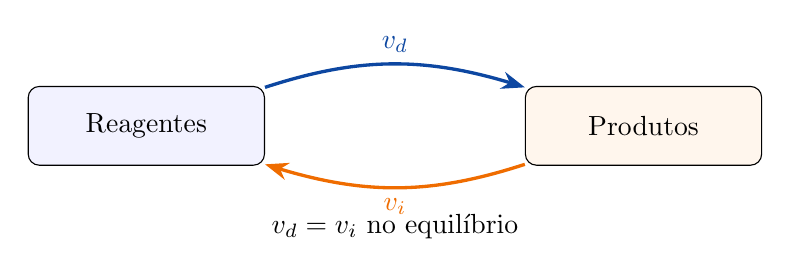
\begin{tikzpicture}[node distance=3.3cm,>=Stealth]
\node[draw,rounded corners,fill=blue!5,minimum width=3cm,minimum height=1cm] (r) {Reagentes};
\node[draw,rounded corners,fill=orange!7,right=of r,minimum width=3cm,minimum height=1cm] (p) {Produtos};
\draw[->,very thick,eublue,bend left=18] (r) to node[above] {$v_d$} (p);
\draw[->,very thick,euorange,bend left=18] (p) to node[below] {$v_i$} (r);
\node[below=1cm of $(r)!0.5!(p)$] {$v_d=v_i$ no equilíbrio};
\end{tikzpicture}
\end{center}

\section{Constante de equilíbrio}
Para $a\ce{A}+b\ce{B}<=>c\ce{C}+d\ce{D}$, em solução homogénea,
\[
\Kc=\frac{[\ce C]^c[\ce D]^d}{[\ce A]^a[\ce B]^b}.
\]
Cada concentração é a de equilíbrio. Substâncias sólidas puras e líquidos puros não aparecem na expressão. A constante depende da temperatura. Um valor muito grande favorece produtos; um valor muito pequeno favorece reagentes, sem significar que a reação seja necessariamente rápida ou lenta.

\begin{exemplo}[title=Exemplo resolvido — cálculo de $\Kc$]
Para \ce{H2(g) + I2(g) <=> 2HI(g)}, as concentrações de equilíbrio são, em \si{mol.dm^{-3}}, $[\ce{H2}]=0,20$, $[\ce{I2}]=0,20$ e $[\ce{HI}]=1,20$. Logo,
\[
\Kc=\frac{(1,20)^2}{0,20\times0,20}=36.
\]
À mesma temperatura, para a reação inversa, $K_{\mathrm{c,inv}}=1/36=2,8\times10^{-2}$.
\end{exemplo}

\section{Tabelas de variação}
Uma tabela inicial--variação--equilíbrio organiza a estequiometria. Considere \ce{N2O4(g) <=> 2NO2(g)} com concentração inicial $c_0$ de \ce{N2O4} e nenhuma de \ce{NO2}. Se se dissociar $x$:
\[
\begin{array}{c|cc}
&\ce{N2O4}&\ce{NO2}\\ \hline
\text{inicial}&c_0&0\\
\text{variação}&-x&+2x\\
\text{equilíbrio}&c_0-x&2x
\end{array}
\qquad
\Kc=\frac{(2x)^2}{c_0-x}.
\]

\begin{exemplo}[title=Exemplo resolvido — concentração de equilíbrio]
Num recipiente, $[\ce{N2O4}]_0=\SI{0.100}{mol.dm^{-3}}$ e, no equilíbrio, $[\ce{NO2}]=\SI{0.060}{mol.dm^{-3}}$. Como $2x=0,060$, $x=0,030$. Assim, $[\ce{N2O4}]_e=0,100-0,030=\SI{0.070}{mol.dm^{-3}}$ e $\Kc=(0,060)^2/0,070=5,1\times10^{-2}$.
\end{exemplo}

\section{Quociente da reação}
O quociente $Q_c$ tem a mesma forma de $\Kc$, mas usa as concentrações num instante qualquer:
\begin{itemize}
  \item $Q_c<\Kc$: evolução no sentido direto;
  \item $Q_c>\Kc$: evolução no sentido inverso;
  \item $Q_c=\Kc$: sistema em equilíbrio.
\end{itemize}

\begin{exemplo}[title=Exemplo resolvido — sentido da evolução]
Para \ce{H2 + I2 <=> 2HI}, $\Kc=36$. Se $[\ce{H2}]=0,40$, $[\ce{I2}]=0,20$ e $[\ce{HI}]=0,80$, então $Q_c=0,80^2/(0,40\times0,20)=8$. Como $Q_c<\Kc$, haverá consumo de \ce{H2} e \ce{I2} e formação de \ce{HI}.
\end{exemplo}

\section{Princípio de Le Châtelier}
Quando um sistema em equilíbrio é perturbado, evolui no sentido que tende a contrariar a perturbação:
\begin{itemize}
  \item aumentar a concentração de um reagente favorece o seu consumo;
  \item aumentar a pressão por diminuição do volume favorece o lado com menor quantidade total de gás;
  \item aumentar a temperatura favorece o sentido endotérmico;
  \item um catalisador acelera igualmente os dois sentidos: reduz o tempo para atingir o equilíbrio, mas não altera $\Kc$ nem a composição de equilíbrio.
\end{itemize}

\section{Síntese do amoníaco: compromissos de engenharia}
Na reação exotérmica \ce{N2(g) + 3H2(g) <=> 2NH3(g)}, pressão elevada favorece o amoníaco e temperatura baixa favorece o sentido exotérmico. Contudo, uma temperatura demasiado baixa torna a reação lenta. Industrialmente usa-se um compromisso de temperatura, pressão elevada, catalisador e remoção/recirculação de substâncias. Termodinâmica, cinética, segurança, custo energético e materiais do reator têm de ser considerados em conjunto.

\begin{atividade}[title=Perturbação do equilíbrio entre ferro(III) e tiocianato]
\textbf{Sistema:} \ce{Fe^{3+}(aq) + SCN^-(aq) <=> FeSCN^{2+}(aq)}, cuja espécie produto apresenta cor vermelha.

\textbf{Questão:} como varia a posição de equilíbrio quando se adiciona um dos iões ou quando se remove \ce{Fe^{3+}} por reação com outra espécie?

Preparar uma solução muito diluída do sistema e distribuir por tubos. Manter um tubo como controlo. Adicionar, em microescala, solução contendo \ce{Fe^{3+}} a um tubo, \ce{SCN^-} a outro e um reagente indicado pelo professor que reduza a concentração de uma das espécies num terceiro. Registar a cor, formular previsões antes de cada adição e interpretar por $Q_c$ e Le Châtelier.

\textbf{Qualidade dos dados:} usar volumes iguais, fundo branco e, se possível, uma aplicação de colorimetria calibrada. Não confundir intensidade de cor com prova quantitativa sem calibração.
\end{atividade}

\begin{seguranca}
Realizar em microescala. As soluções de ferro(III) e de tiocianato são irritantes/nocivas consoante a concentração. Usar proteção ocular, evitar contacto e recolher resíduos em recipiente próprio.
\end{seguranca}

\begin{exercicios}[title=Exercícios do capítulo 6]
\begin{enumerate}[label=6.\arabic*.]
  \item Escreve $\Kc$ para: (a) \ce{2SO2(g) + O2(g) <=> 2SO3(g)}; (b) \ce{CaCO3(s) <=> CaO(s) + CO2(g)}.
  \item Para \ce{A(g) <=> 2B(g)}, $[\ce A]_e=0,50$ e $[\ce B]_e=0,30$ em \si{mol.dm^{-3}}. Calcula $\Kc$.
  \item Para \ce{2SO2 + O2 <=> 2SO3}, $\Kc=4,0$. Num estado, as concentrações são $0,50$, $0,50$ e $0,20$ \si{mol.dm^{-3}}, respetivamente. Prevê o sentido de evolução.
  \item Indica o efeito de diminuir o volume no equilíbrio \ce{N2O4(g) <=> 2NO2(g)}.
  \item Numa reação exotérmica em equilíbrio, explica o efeito de elevar a temperatura sobre $\Kc$ e sobre a quantidade de produto.
  \item Explica por que motivo um catalisador não aumenta o rendimento de equilíbrio do processo de Haber, embora seja essencial industrialmente.
\end{enumerate}
\end{exercicios}

% =========================================================
\part{Física — Mecânica}
% =========================================================

\chapter{Tempo, posição, velocidade e aceleração}
\begin{objetivos}
\begin{itemize}
  \item descrever movimentos relativamente a um referencial;
  \item distinguir posição, distância percorrida e deslocamento;
  \item interpretar velocidade e aceleração como grandezas vetoriais;
  \item analisar gráficos posição--tempo e velocidade--tempo;
  \item classificar movimentos retilíneos;
  \item recolher e analisar dados de movimentos reais.
\end{itemize}
\end{objetivos}

\section{Referencial, trajetória e posição}
Movimento e repouso dependem do referencial. Um passageiro sentado está em repouso relativamente ao comboio, mas em movimento relativamente ao solo. Num movimento unidimensional, escolhem-se uma origem e um sentido positivo; a posição $x$ pode ser positiva, nula ou negativa.

O deslocamento é
\[
\Delta x=x_f-x_i.
\]
É uma grandeza vetorial e, em uma dimensão, o sinal representa o sentido. A distância percorrida é escalar e soma comprimentos ao longo da trajetória; por isso, pode ser maior que $|\Delta x|$.

\begin{exemplo}[title=Exemplo resolvido — distância e deslocamento]
Um atleta corre de $x=\SI{10}{m}$ até $x=\SI{70}{m}$ e regressa a $x=\SI{30}{m}$. A distância é $60+40=\SI{100}{m}$; o deslocamento é $30-10=+\SI{20}{m}$.
\end{exemplo}

\section{Velocidade média e velocidade}
A velocidade média num intervalo é
\[
v_m=\frac{\Delta x}{\Delta t}.
\]
A velocidade num instante corresponde à taxa de variação da posição e, num gráfico $x(t)$, ao declive da tangente. O vetor velocidade é sempre tangente à trajetória. A rapidez é o módulo da velocidade.

\section{Aceleração}
A aceleração média é
\[
a_m=\frac{\Delta v}{\Delta t}.
\]
Uma aceleração positiva não significa necessariamente aumento de rapidez: a rapidez aumenta quando velocidade e aceleração têm o mesmo sentido e diminui quando têm sentidos opostos.

\begin{table}[h!]
\centering
\caption{Sinal de $v$ e $a$ num movimento retilíneo.}
\begin{tabular}{ccc}
\toprule
$v$ e $a$ & Efeito na rapidez & Classificação local \\
\midrule
mesmo sinal & aumenta & acelerado \\
sinais opostos & diminui & retardado \\
$a=0$ & constante & uniforme \\
\bottomrule
\end{tabular}
\end{table}

\section{Leitura de gráficos}
Num gráfico $x(t)$, o declive dá a velocidade. Num gráfico $v(t)$, o declive dá a aceleração e a área algébrica entre o gráfico e o eixo do tempo dá o deslocamento.

\begin{center}
\begin{tikzpicture}
\begin{axis}[width=.72\textwidth,height=5.8cm,axis lines=middle,xlabel={$t$/s},ylabel={$v$/\si{m.s^{-1}}},xmin=0,xmax=8,ymin=-2,ymax=7,grid=both]
\addplot[eublue,very thick] coordinates {(0,2)(4,6)(6,6)(8,0)};
\end{axis}
\end{tikzpicture}
\end{center}
Entre 0 e \SI{4}{s}, a aceleração é positiva; entre 4 e \SI{6}{s}, é nula; depois é negativa. A interpretação “aceleração negativa = travagem” só é correta se $v$ for positiva nesse intervalo.

\begin{exemplo}[title=Exemplo resolvido — área num gráfico $v(t)$]
Um corpo parte com $v_0=\SI{2.0}{m.s^{-1}}$ e atinge $v=\SI{8.0}{m.s^{-1}}$ uniformemente em \SI{3.0}{s}. O deslocamento é a área do trapézio:
\[
\Delta x=\frac{2,0+8,0}{2}\times3,0=\SI{15}{m}.
\]
A aceleração é $(8,0-2,0)/3,0=\SI{2.0}{m.s^{-2}}$.
\end{exemplo}

\section{Equações do movimento uniformemente variado}
Quando $a$ é constante,
\[
v=v_0+at,
\qquad
x=x_0+v_0t+\frac12at^2,
\qquad
v^2=v_0^2+2a\Delta x.
\]
Estas equações não devem ser usadas quando a aceleração varia significativamente.

\begin{atividade}[title=Aquisição de dados de um movimento real]
Usa um sensor de posição, vídeo com escala ou aplicação adequada para registar $x(t)$ de um carrinho ou pessoa. Define o referencial antes da recolha. Obtém gráficos $x(t)$ e $v(t)$, identifica intervalos de movimento aproximadamente uniforme/acelerado/retardado e compara velocidades calculadas por diferenças finitas com o declive do gráfico.

\textbf{Avaliação:} discutir taxa de amostragem, paralaxe, calibração da escala, suavização excessiva dos dados e escolha do intervalo de ajuste.
\end{atividade}

\begin{exercicios}[title=Exercícios do capítulo 7]
\begin{enumerate}[label=7.\arabic*.]
  \item Um móvel passa de $x=-\SI{4}{m}$ para $x=\SI{11}{m}$ em \SI{5}{s}. Calcula deslocamento e velocidade média.
  \item Um automóvel com $v=\SI{20}{m.s^{-1}}$ trava com $a=-\SI{4.0}{m.s^{-2}}$. Calcula o tempo e a distância de travagem, admitindo aceleração constante.
  \item Um gráfico $v(t)$ é triangular: $v$ cresce de 0 a \SI{12}{m.s^{-1}} em \SI{4}{s} e regressa a zero nos \SI{2}{s} seguintes. Determina o deslocamento total.
  \item Dá um exemplo em que $v<0$ e $a<0$ e interpreta a variação da rapidez.
  \item Explica por que a área sob um gráfico aceleração--tempo representa variação de velocidade e não deslocamento.
\end{enumerate}
\end{exercicios}

\section{Aprofundamento — gráficos e descrição de movimentos}
\begin{metodo}[title=Ler gráficos sem confundir trajetória e representação]
Uma linha num gráfico posição--tempo representa pares $(t,x)$ e não o
caminho geométrico seguido pelo corpo. Para extrair informação:
\begin{enumerate}
\item lê $x_i$ e $x_f$ e calcula $\Delta x=x_f-x_i$;
\item determina a velocidade média pelo declive da secante;
\item determina a velocidade instantânea pelo declive da tangente;
\item assinala máximos ou mínimos de $x(t)$ que possam corresponder a
inversões do sentido do movimento.
\end{enumerate}
Uma tangente horizontal num instante informa que $v=0$ nesse instante;
não prova que o móvel permaneceu em repouso durante um intervalo.
\end{metodo}
\begin{center}
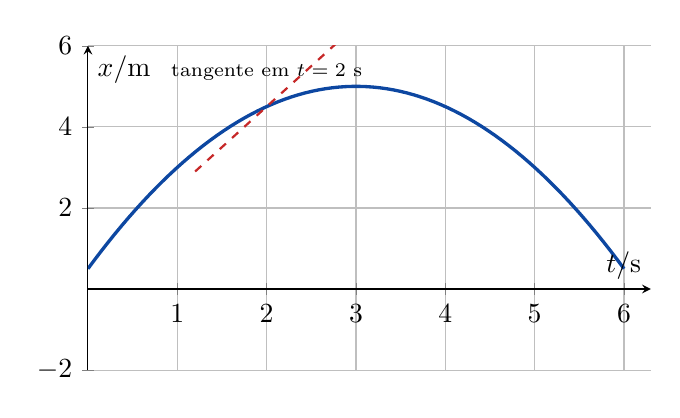
\begin{tikzpicture}
\begin{axis}[width=.72\textwidth,height=5.7cm,axis lines=middle,
xlabel={$t$/s},ylabel={$x$/m},xmin=0,xmax=6.3,ymin=-2,ymax=6,
xtick={0,1,2,3,4,5,6},grid=both]
\addplot[eublue,very thick,domain=0:6,samples=80]{-0.5*(x-3)^2+5};
\addplot[eured,dashed,thick,domain=1.2:3]{2*x+0.5};
\node at (axis cs:2,5.35) {\scriptsize tangente em $t=2$ s};
\end{axis}
\end{tikzpicture}
\end{center}
No exemplo desenhado, $x(t)=-\tfrac12(t-3)^2+5$, pelo que
$v(t)=3-t$. Entre 0 e 3 s, $v>0$; aos 3 s, $v=0$; depois,
$v<0$. A tangente vermelha no instante 2 s tem declive
$+\SI{1}{m.s^{-1}}$.
\begin{nota}
Num gráfico $v(t)$, o deslocamento é a \emph{área algébrica}
$\int v\,\mathrm dt$. A distância percorrida é a soma dos módulos das
áreas. Se uma área estiver abaixo do eixo dos tempos, contribui
negativamente para $\Delta x$ e positivamente para a distância.
\end{nota}


\section{Do registo de posições à descrição completa do movimento}
O resumo original acompanha uma deslocação através de posições sucessivas,
uma tabela horária e um gráfico. Uma fotografia informa sobre a posição num
instante; uma tabela reúne medições discretas; um gráfico permite comparar
intervalos e estimar tendências. A linha que liga os pontos medidos representa
uma interpolação ou um modelo que deve ser confrontado com os dados.
\begin{table}[H]
\centering
\caption{Registo de uma posição vertical em intervalos iguais.}
\begin{tabular}{@{}lccccc@{}}\toprule
$t$/s & $0,0$ & $0,2$ & $0,4$ & $0,6$ & $0,8$\\
\midrule
$y$/m & $3,1$ & $2,9$ & $2,4$ & $1,4$ & $0,0$\\
\bottomrule\end{tabular}
\end{table}
Entre o primeiro e o último registo, $\Delta y=-\SI{3.1}{m}$ e a
componente da velocidade média é
$\bar v_y=-3,1/0,8=-\SI{3.875}{m.s^{-1}}$.
Se não houver inversão, a rapidez média vale \SI{3.875}{m.s^{-1}}.
Os deslocamentos em intervalos iguais têm módulos $0,2$, $0,5$,
$1,0$ e $1,4$ m: a rapidez cresce. Como as diferenças não são
exatamente constantes, o modelo de aceleração constante é
aproximado e deve considerar a incerteza de medição.
\begin{metodo}[title=Leitura de sinais em gráficos]
\begin{itemize}
\item Em $x(t)$, uma curva crescente significa $v_x>0$;
decrescente, $v_x<0$; uma tangente horizontal significa $v_x=0$
nesse instante, não necessariamente repouso duradouro.
\item Em $v_x(t)$, o sinal da ordenada indica o sentido do movimento
e o declive dá a aceleração.
\item A passagem de $v_x$ por zero pode assinalar inversão se os
sinais antes e depois forem diferentes.
\item O deslocamento soma as áreas com sinal; a distância soma os
módulos das áreas entre $v_x(t)$ e o eixo do tempo.
\end{itemize}
\end{metodo}
\begin{center}
\begin{tikzpicture}
\begin{axis}[width=.75\textwidth,height=5.5cm,xmin=0,xmax=6,
ymin=-3,ymax=4,xlabel={$t$/s},ylabel={$v_x$/\si{m.s^{-1}}},
grid=both,axis lines=middle]
\addplot[eublue,very thick] coordinates {(0,0)(2,3)(4,3)(5,0)(6,-2)};
\node[font=\scriptsize] at (axis cs:3,3.45) {área positiva};
\node[font=\scriptsize] at (axis cs:5.4,-1.8) {área negativa};
\end{axis}
\end{tikzpicture}
\end{center}
As quatro áreas, por ordem, são $+3$, $+6$, $+1,5$ e $-1$ m.
Logo $\Delta x=\SI{9.5}{m}$, mas $d=\SI{11.5}{m}$.
\begin{exemplo}[title=Exemplo resolvido — secante e tangente]
Para $x(t)=2+3t-t^2$ (SI), a velocidade média entre 0 e 2 s é
$[x(2)-x(0)]/2=(4-2)/2=\SI{1}{m.s^{-1}}$.
No instante 2 s, o declive da tangente é
$v_x=3-2t=-\SI{1}{m.s^{-1}}$. A velocidade média positiva é
compatível com a velocidade final negativa porque ocorreu uma
inversão em $t=\SI{1.5}{s}$.
\end{exemplo}


\begin{nota}
As fichas desta secção e dos capítulos seguintes adaptam os materiais
\textit{Fichas 11 Ano.tex}, \textit{Resolução Fichas 11 Ano.tex} e
\textit{Física: Resumo 11.º ano} de José Gonçalves. Os enunciados que
exigiam imagens externas foram reformulados com dados completos e
esquemas TikZ. Nas resoluções, compara o método com o teu antes de
consultar o resultado; justifica sempre os sinais e as unidades.
\end{nota}

\section{Ficha 1 — Mecânica: referencial e interpretação}
\begin{exercicios}[title=Questões da ficha 1]
\begin{enumerate}[label=F1.\arabic*.]
\item Uma esfera desloca-se no sentido negativo de $Ox$ com aceleração
constante. Em quatro intervalos de tempo iguais, as distâncias sucessivas
são proporcionais a $1:3:5:7$. Sabendo que percorre \SI{50}{cm} no último,
determina a distância nos três primeiros e indica os sentidos de $\vect v$
e $\vect a$.
\item Um carrinho passa de $x=\SI{3}{m}$ a $x=-\SI{9}{m}$, regressando a
$x=\SI{-2}{m}$. Calcula deslocamento e distância total. Pode a rapidez média
ser calculada só com o deslocamento?
\item Um gráfico $v_x(t)$ é constituído por três troços: $v=0$ de 0 a
\SI{1}{s}; aumento linear de 0 a \SI{0.8}{m.s^{-1}} entre 1 e \SI{2}{s};
$v=\SI{0.8}{m.s^{-1}}$ de 2 a \SI{3}{s}. Determina aceleração no segundo
troço e deslocamento total.
\end{enumerate}
\end{exercicios}

\begin{center}
\begin{tikzpicture}
\begin{axis}[width=.78\textwidth,height=5cm,xmin=0,xmax=3.4,ymin=0,ymax=1.05,
 xlabel={$t$/s},ylabel={$v_x$/\si{m.s^{-1}}},grid=both]
\addplot[eublue,very thick] coordinates {(0,0)(1,0)(2,.8)(3,.8)};
\end{axis}
\end{tikzpicture}
\end{center}

\begin{solucao}[title=Ficha 1]
\textbf{F1.1} A unidade da razão é $50/7$ cm. As três distâncias
são $50/7$, $150/7$ e $250/7$ cm; a soma é
$450/7\approx\SI{64.3}{cm}$. Se a esfera acelera no sentido negativo,
$\vect v$ e $\vect a$ têm ambos esse sentido.\par
\textbf{F1.2} $\Delta x=-2-3=-\SI{5}{m}$;
$d=|{-9}-3|+|{-2}-({-9})|=12+7=\SI{19}{m}$.
A rapidez média requer $d/\Delta t$.\par
\textbf{F1.3} $a=\Delta v/\Delta t=\SI{0.8}{m.s^{-2}}$;
$\Delta x=0+\frac12(1)(0.8)+(1)(0.8)=\SI{1.2}{m}$.
\end{solucao}

\section{Ficha 2 — Tempo, posição, velocidade e aceleração}
\begin{exercicios}[title=Questões da ficha 2]
\begin{enumerate}[label=F2.\arabic*.]
\item Um corredor parte do repouso em $x_0=-\SI{5}{m}$, acelera
uniformemente durante \SI{4}{s} e percorre \SI{16}{m}. Mantém depois
\SI{8}{m.s^{-1}} durante \SI{6}{s} e trava uniformemente durante
\SI{3}{s} até parar. Determina $a$ nos dois intervalos não uniformes,
$x(\SI{5}{s})$, a distância total e o módulo da velocidade média global.
\item Esboça $v_x(t)$ para o corredor e explica como obter a distância
total pelas áreas. Identifica o instante em que $x=\SI{11}{m}$.
\item Uma bola é largada do repouso. Orienta $Oy$ para cima e adota
$g=\SI{10}{m.s^{-2}}$. Escreve $y(t)$ para $y_0=\SI{20}{m}$;
determina $v_y$ aos \SI{1.5}{s} e o instante em que atinge o solo.
\end{enumerate}
\end{exercicios}

\begin{solucao}[title=Ficha 2]
\textbf{F2.1} $a_1=8/4=\SI{2}{m.s^{-2}}$;
$a_3=(0-8)/3=-\SI{2.67}{m.s^{-2}}$.
$x(5)=-5+16+8=\SI{19}{m}$. Na travagem percorre
$(8+0)3/2=\SI{12}{m}$; distância total $16+48+12=\SI{76}{m}$;
rapidez e módulo da velocidade média (sem inversão) $76/13=\SI{5.85}{m.s^{-1}}$.\par
\textbf{F2.2} Une os pontos $(t,v)=(0,0),(4,8),(10,8),(13,0)$;
as áreas são triângulo de \SI{16}{m}, retângulo de \SI{48}{m} e
triângulo de \SI{12}{m}. $x=11$ m aos \SI{4}{s}.\par
\textbf{F2.3} $y(t)=20-5t^2$ (SI); $v_y(t)=-10t$;
$v_y(1.5)=-\SI{15}{m.s^{-1}}$; $t=\sqrt{4}=\SI{2}{s}$.
\end{solucao}

\chapter{Interações, Leis de Newton e gravitação}
\begin{objetivos}
\begin{itemize}
  \item reconhecer força como descrição de uma interação;
  \item identificar as quatro interações fundamentais e as suas escalas;
  \item construir diagramas de forças;
  \item aplicar as três Leis de Newton;
  \item aplicar a Lei da Gravitação Universal;
  \item determinar experimentalmente a aceleração gravítica.
\end{itemize}
\end{objetivos}

\section{As quatro interações fundamentais}
Gravitacional, eletromagnética, nuclear forte e nuclear fraca constituem as interações fundamentais conhecidas. A gravitação tem alcance ilimitado e domina a estrutura astronómica apesar da sua fraca intensidade microscópica. A interação eletromagnética também tem alcance ilimitado e explica contacto, atrito, elasticidade e química. As interações forte e fraca atuam a escalas subatómicas.

\section{Força resultante e diagramas}
Uma força não é propriedade isolada de um corpo: representa a interação entre corpos. Num diagrama, isola-se o corpo e representam-se apenas as forças que atuam nele. Peso e força normal não formam um par ação--reação, porque atuam no mesmo corpo.

\begin{center}
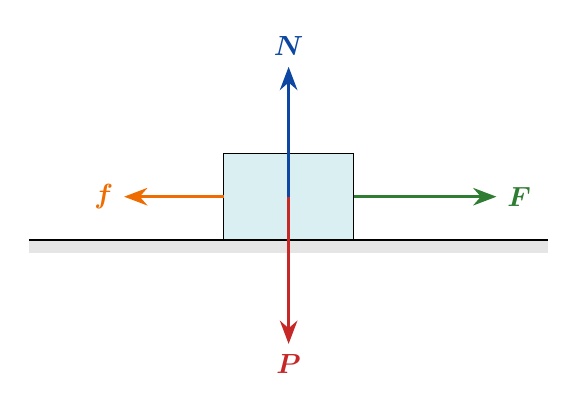
\begin{tikzpicture}[>=Stealth,scale=1.1]
\fill[gray!20] (-3,-.15) rectangle (3,0);
\draw[thick] (-3,0)--(3,0);
\draw[fill=eucyan!15] (-.75,0) rectangle (.75,1);
\draw[->,very thick,eublue] (0,.5)--(0,2) node[above] {$\vect N$};
\draw[->,very thick,eured] (0,.5)--(0,-1.2) node[below] {$\vect P$};
\draw[->,very thick,eugreen] (.75,.5)--(2.4,.5) node[right] {$\vect F$};
\draw[->,very thick,euorange] (-.75,.5)--(-1.9,.5) node[left] {$\vect f$};
\end{tikzpicture}
\end{center}

\section{Leis de Newton}
\begin{enumerate}
  \item Se $\sum\vect F=\vect0$, a velocidade permanece constante; repouso é um caso particular.
  \item $\sum\vect F=m\vect a$ para um corpo de massa constante num referencial inercial.
  \item As forças de interação entre dois corpos têm igual intensidade, mesma direção e sentidos opostos, atuando em corpos diferentes.
\end{enumerate}

\begin{exemplo}[title=Exemplo resolvido — corpo puxado com atrito]
Uma caixa de \SI{12}{kg} é puxada horizontalmente por \SI{50}{N}; o atrito vale \SI{14}{N}. A resultante horizontal é \SI{36}{N} e
\[
a=\frac{36}{12}=\SI{3.0}{m.s^{-2}}.
\]
Verticalmente, sem aceleração, $N=mg$.
\end{exemplo}

\section{Gravitação universal}
Dois corpos de massas $m_1$ e $m_2$, separados por $r$, atraem-se com
\[
F_g=G\frac{m_1m_2}{r^2}.
\]
Perto da superfície de um astro, $g=GM/r^2$ e $P=mg$. A massa é propriedade do corpo; o peso depende do campo gravítico local.

\begin{exemplo}[title=Exemplo resolvido — gravidade a uma altitude]
À altitude $h=R_T$, a distância ao centro da Terra é $2R_T$. Portanto,
\[
g_h=\frac{GM_T}{(2R_T)^2}=\frac{g_0}{4}\approx\SI{2.45}{m.s^{-2}}.
\]
\end{exemplo}

\section{Determinação experimental de \texorpdfstring{$g$}{g} por queda livre}
Sem resistência do ar apreciável, um corpo largado tem $y=y_0+\tfrac12gt^2$ se o sentido positivo for para baixo. Medir apenas um tempo para uma altura pequena amplifica o efeito do tempo de reação; sensores, eletroímanes, fotocélulas ou análise de vídeo reduzem esse problema.

\begin{atividade}[title=A aceleração gravítica depende da massa?]
\textbf{Questão:} dentro da incerteza, corpos de massas diferentes apresentam a mesma aceleração em queda?

Filmar a queda de dois objetos compactos de forma semelhante diante de uma escala vertical, com câmara fixa e elevada taxa de imagens. Extrair $y(t)$ e ajustar $y=y_0+v_0t+\tfrac12at^2$. Repetir, estimar incerteza e comparar os intervalos de $a$.

\textbf{Cuidados:} zona de queda desimpedida, proteção do solo/objetos, câmara perpendicular ao plano de movimento, escala no mesmo plano e altura que torne a resistência do ar pouco relevante.
\end{atividade}

\enlargethispage{2\baselineskip}
\begin{exercicios}[title=Exercícios do capítulo 8]
\begin{enumerate}[label=8.\arabic*.]
  \item Uma resultante de \SI{18}{N} atua num corpo de \SI{6.0}{kg}. Calcula a aceleração.
  \item Um bloco de \SI{4.0}{kg} está num plano horizontal com $\mu=0,20$. É puxado por \SI{15}{N}. Admite $g=\SI{9.8}{m.s^{-2}}$ e calcula a aceleração.
  \item Explica por que ação e reação não se anulam no diagrama de forças de um único corpo.
  \item Um planeta tem massa $2M_T$ e raio $1,5R_T$. Determina $g/g_T$.
  \item Num gráfico de $y$ em função de $t^2$, o declive é \SI{4.86}{m.s^{-2}}. Determina $g$.
\end{enumerate}
\end{exercicios}

\section{Aprofundamento — interação, força e aceleração}
Para analisar um sistema, começa por escolher o corpo de interesse.
Cada seta num diagrama de forças representa uma força \emph{exercida sobre
esse corpo} por outro corpo. Duas forças da terceira lei de Newton
atuam sobre \emph{corpos diferentes}; por isso, não se cancelam no
diagrama de forças de um só corpo.
\begin{center}
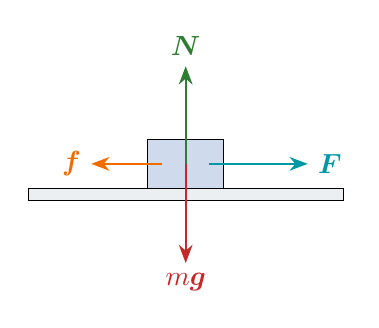
\begin{tikzpicture}[>=Stealth,scale=1]
\draw[fill=eugrey] (-2,-.15) rectangle (2,0);
\draw[fill=eublue!20] (-.48,0) rectangle (.48,.62);
\draw[->,thick,eugreen] (0,.31)--(0,1.55) node[above] {$\vect N$};
\draw[->,thick,eured] (0,.31)--(0,-.95) node[below] {$m\vect g$};
\draw[->,thick,eucyan] (.3,.31)--(1.55,.31) node[right] {$\vect F$};
\draw[->,thick,euorange] (-.3,.31)--(-1.2,.31) node[left] {$\vect f$};
\end{tikzpicture}
\end{center}
Quando a velocidade e a força resultante são colineares, a força
pode aumentar ou diminuir a rapidez. Se a resultante tiver uma
componente perpendicular à velocidade, muda a direção do movimento.
No limite em que só existe componente perpendicular, o módulo de
$\vect v$ mantém-se constante, mas $\vect v$ varia e a aceleração
é diferente de zero.
\begin{exemplo}[title=Exemplo resolvido — massa a partir de um gráfico]
Um gráfico $F_{\mathrm R}(a)$ é uma reta pela origem que passa por
$(\SI{2}{m.s^{-2}},\SI{6}{N})$. O declive é
$m=F_{\mathrm R}/a=\SI{3}{kg}$. Se a mesma força atuar num corpo
de massa dupla, a aceleração reduz-se para metade.
\end{exemplo}
\begin{stem}
Constrói uma rampa e mede $a$ de um carrinho com vídeo. Repete
com duas massas, mantendo aproximadamente a mesma força motora.
Representa $F_{\mathrm R}$ em função de $a$ e estima a massa pelo
declive. Indica o papel do atrito e da incerteza da escala espacial.
\end{stem}


\section{Interações e decomposição da resultante}
\begin{table}[H]
\centering\small
\caption{As quatro interações fundamentais.}
\begin{tabularx}{\textwidth}{@{}p{.24\textwidth}p{.26\textwidth}X@{}}
\toprule
Interação & Alcance qualitativo & Exemplo\\\midrule
Gravítica & longo alcance & queda e órbita\\
Eletromagnética & longo alcance & cargas, ímanes, ligações químicas\\
Nuclear forte & escala nuclear & coesão dos nucleões\\
Nuclear fraca & escala subatómica & alguns decaimentos radioativos\\
\bottomrule\end{tabularx}
\end{table}
Uma força caracteriza-se por módulo, direção, sentido e ponto de aplicação.
No modelo de partícula material representamo-la aplicada no centro de
massa; para corpos extensos sujeitos a rotação ou deformação o ponto de
aplicação volta a ser importante.
Na terceira lei, $\vect F_{A\to B}=-\vect F_{B\to A}$:
as forças atuam em corpos diferentes. O peso de uma bola é a força da
Terra sobre a bola; a reação é a força da bola sobre a Terra.
O peso e a normal de apoio podem anular a resultante sobre a bola, mas
não são um par da terceira lei.

\begin{center}
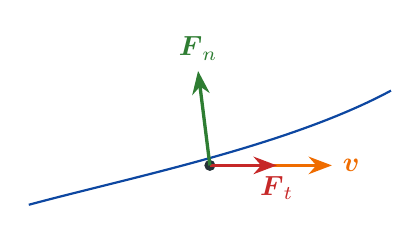
\begin{tikzpicture}[>=Stealth]
\draw[eublue,thick] (-2.3,-.35) .. controls (-1,0) and (1,.4) .. (2.3,1.1);
\fill[eudark] (0,.15) circle (2pt);
\draw[->,very thick,euorange] (0,.15)--(1.55,.15)
 node[right] {$\vect v$};
\draw[->,very thick,eured] (0,.15)--(.85,.15)
 node[below] {$\vect F_t$};
\draw[->,very thick,eugreen] (0,.15)--(-.15,1.35)
 node[above] {$\vect F_n$};
\end{tikzpicture}
\end{center}
Decompõe a resultante em componente tangencial e normal:
$\vect F_{\mathrm R}=\vect F_t+\vect F_n$. A primeira altera o
módulo da velocidade; a segunda altera a sua direção.
Numa trajetória de raio local $r$, a componente normal tem
módulo $F_n=mv^2/r$ e aponta para o centro de curvatura.
A aceleração tem a direção da resultante, que pode diferir
da direção da velocidade.
\begin{mundo}
Quando um autocarro trava, o passageiro tende a manter a velocidade
anterior. O cinto e os apoios exercem forças que a alteram. Esta
tendência de conservação do movimento é a inércia; maior massa
significa maior resistência a uma mesma aceleração.
\end{mundo}


\section{Ficha 3 — Interações e os seus efeitos}
\begin{exercicios}[title=Questões da ficha 3]
\begin{enumerate}[label=F3.\arabic*.]
\item Identifica a interação responsável por (a) um satélite permanecer
em órbita, (b) um íman atrair um clip metálico, (c) manter protões e
neutrões unidos no núcleo e (d) certos processos de decaimento radioativo.
\item Um bloco de \SI{2}{kg} repousa numa mesa horizontal. Desenha o
diagrama de forças, indica os respetivos agentes e determina a reação normal,
admitindo $g=\SI{10}{m.s^{-2}}$.
\item Sobre um carrinho de \SI{0.5}{kg} atuam duas forças horizontais
opostas, de \SI{4}{N} para a direita e \SI{1.5}{N} para a esquerda.
Determina a aceleração e distingue o par ação--reação destas duas forças.
\end{enumerate}
\end{exercicios}

\begin{solucao}[title=Ficha 3]
\textbf{F3.1} (a) gravítica; (b) eletromagnética;
(c) nuclear forte; (d) nuclear fraca.\par
\textbf{F3.2} Peso $P=mg=\SI{20}{N}$ para baixo e normal
$N=\SI{20}{N}$ para cima. Ambos atuam sobre o bloco, logo não formam
um par ação--reação.\par
\textbf{F3.3} $F_R=4-1.5=\SI{2.5}{N}$ para a direita;
$a=F_R/m=\SI{5}{m.s^{-2}}$. As duas forças atuam no mesmo carrinho,
por isso não constituem par ação--reação; cada reação atua no agente
que exerceu a força correspondente.
\end{solucao}

\chapter{Forças e movimentos}
\begin{objetivos}
\begin{itemize}
  \item relacionar resultante, condições iniciais e tipo de movimento;
  \item resolver problemas de movimento retilíneo e em plano inclinado;
  \item interpretar queda com resistência do ar e velocidade terminal;
  \item caracterizar movimento circular uniforme;
  \item aplicar gravitação e dinâmica a satélites;
  \item investigar resultante nula/não nula e a relação $v^2(\Delta x)$.
\end{itemize}
\end{objetivos}

\section{Condições iniciais e resultante}
Conhecer a aceleração não basta: as condições iniciais determinam a evolução. Com resultante nula, a velocidade é constante. Com resultante constante, a aceleração é constante. Uma força pode alterar o módulo da velocidade, a direção ou ambos.

\section{Plano inclinado}
Num plano de ângulo $\theta$, o peso decompõe-se em $mg\sin\theta$ paralelamente ao plano e $mg\cos\theta$ perpendicularmente. Sem aceleração normal, $N=mg\cos\theta$; com atrito cinético idealizado, $f=\mu N$.

\begin{center}
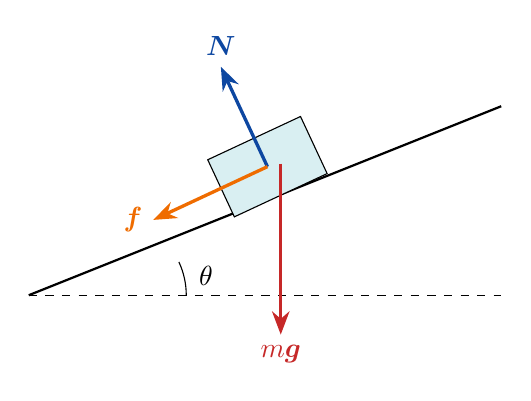
\begin{tikzpicture}[>=Stealth,scale=1.0]
\coordinate (O) at (0,0);
\draw[thick] (-1,0)--(5,2.4);
\draw[dashed] (-1,0)--(5,0);
\draw (1,0) arc[start angle=0,end angle=25,radius=1];
\node at (1.25,.25) {$\theta$};
\begin{scope}[shift={(2.2,1.27)},rotate=25]
\draw[fill=eucyan!15] (-.65,0) rectangle (.65,.8);
\draw[->,very thick,eublue] (0,.4)--(0,1.8) node[above] {$\vect N$};
\draw[->,very thick,euorange] (0,.4)--(-1.6,.4) node[left] {$\vect f$};
\end{scope}
\draw[->,very thick,eured] (2.2,1.67)--(2.2,-.5) node[below] {$m\vect g$};
\end{tikzpicture}
\end{center}

\begin{exemplo}[title=Exemplo resolvido — descida num plano]
Um bloco desliza sem atrito num plano com $\theta=30^\circ$. Na direção do plano, $ma=mg\sin\theta$, logo $a=g\sin30^\circ=\SI{4.9}{m.s^{-2}}$. A massa cancela: no modelo sem resistência, a aceleração não depende dela.
\end{exemplo}

\section{Resistência do ar e velocidade terminal}
A resistência do ar depende da forma, área, rapidez e propriedades do fluido. Num corpo em queda, aumenta com a rapidez. Quando iguala o peso, a resultante torna-se nula e a velocidade estabiliza: atinge-se a velocidade terminal. Objetos com grande área relativamente à massa tendem a atingir menor velocidade terminal.

\section{Movimento circular uniforme}
Embora a rapidez seja constante, a velocidade muda de direção. A aceleração centrípeta aponta para o centro:
\[
a_c=\frac{v^2}{r}=\omega^2r,qquad v=\frac{2\pi r}{T}.
\]
“Força centrípeta” não é uma força nova; é o nome da componente radial da resultante das forças reais.

\begin{exemplo}[title=Exemplo resolvido — curva plana]
Um automóvel descreve uma curva de raio \SI{50}{m} a \SI{10}{m.s^{-1}}. A aceleração centrípeta é $a_c=100/50=\SI{2.0}{m.s^{-2}}$. Para massa de \SI{1200}{kg}, a resultante radial necessária é \SI{2.4e3}{N}, fornecida pelo atrito estático pneu--estrada.
\end{exemplo}

\section{Satélites em órbita circular}
Para um satélite de massa $m$ em torno de um astro de massa $M$,
\[
G\frac{Mm}{r^2}=m\frac{v^2}{r}
\Rightarrow v=\sqrt{\frac{GM}{r}},
\]
\[
T=2\pi\sqrt{\frac{r^3}{GM}}.
\]
A massa do satélite cancela. Uma órbita é queda livre contínua: o satélite “cai” em direção ao astro enquanto a superfície se curva para longe.

\begin{exemplo}[title=Exemplo resolvido — comparação de órbitas]
Se o raio orbital passa de $r$ para $4r$, então $v$ passa para $v/2$ e o período para $T\sqrt{4^3}=8T$.
\end{exemplo}

\begin{atividade}[title=Resultante nula e não nula]
Num carrinho de baixo atrito, compara: (A) movimento após um impulso, com força propulsora removida; (B) movimento puxado por massa suspensa aproximadamente constante. Recolhe $v(t)$, ajusta retas em intervalos adequados e associa declive aproximadamente nulo a resultante aproximadamente nula e declive não nulo a resultante não nula.
\end{atividade}

\begin{atividade}[title=Relação entre velocidade e deslocamento]
Faz descer um carrinho num plano inclinado e mede velocidades em diferentes posições. Representa $v^2$ em função de $\Delta x$. Para aceleração constante,
\[
v^2=v_0^2+2a\Delta x,
\]
pelo que o declive é $2a$. Determina $a$ pelo ajuste e $F_R=ma$; compara com a previsão baseada nas forças.
\end{atividade}

\begin{stem}
\textbf{Exploração espacial.} Escolhe uma missão recente ou histórica e analisa: órbita, instrumentos, comunicação, fontes de energia, materiais, risco, lixo espacial e benefício científico/social. Distingue dados da missão, inferências e propostas futuras.
\end{stem}

\begin{exercicios}[title=Exercícios do capítulo 9]
\begin{enumerate}[label=9.\arabic*.]
  \item Um bloco desce sem atrito um plano de $20^\circ$. Calcula a aceleração.
  \item Um corpo parte do repouso e percorre \SI{12}{m} com aceleração \SI{1.5}{m.s^{-2}}. Calcula a velocidade final.
  \item Explica a evolução da aceleração de um paraquedista desde o salto até à velocidade terminal e após abrir o paraquedas.
  \item Um corpo descreve uma circunferência de raio \SI{0.80}{m} com período \SI{1.6}{s}. Calcula rapidez e aceleração centrípeta.
  \item Um satélite orbital tem raio $9R_T$. Compara a sua rapidez e o seu período com os de um satélite de raio $R_T$, no modelo ideal.
  \item Num gráfico $v^2$ em função de $x$, o declive é \SI{3.6}{m.s^{-2}}. Determina a aceleração.
\end{enumerate}
\end{exercicios}

% =========================================================
\section{Aprofundamento — resistência do ar e órbitas}
\begin{center}
\begin{tikzpicture}
\begin{axis}[width=.75\textwidth,height=5.5cm,xmin=0,xmax=9,
ymin=0,ymax=11,xlabel={$t$/s},ylabel={$v$/\si{m.s^{-1}}},
grid=major,legend style={at={(.97,.28)},anchor=east,font=\scriptsize}]
\addplot[eured,dashed,domain=0:9]{10*x};
\addlegendentry{modelo sem ar}
\addplot[eublue,very thick,domain=0:9,samples=80]{8*(1-exp(-.8*x))};
\addlegendentry{modelo com arrasto}
\end{axis}
\end{tikzpicture}
\end{center}
O gráfico azul ilustra apenas um modelo: no início, a velocidade
cresce e a força de resistência do ar aumenta. Quando esta iguala o
peso, a força resultante e a aceleração tornam-se nulas e a
velocidade aproxima-se de um valor terminal. A forma exata da curva
depende do modelo de arrasto; o gráfico não corresponde a dados
experimentais. O modelo tracejado sem ar excede a escala do gráfico
após o primeiro segundo.
\begin{exemplo}[title=Exemplo resolvido — satélite circular]
Da igualdade $GMm/r^2=mv^2/r$ obtém-se
$v=\sqrt{GM/r}$. Como $v=2\pi r/T$, então
$T=2\pi\sqrt{r^3/(GM)}$. A massa do satélite cancela-se.
Ao dobrar $r$, o período multiplica-se por $2^{3/2}$.
\end{exemplo}
\begin{mundo}
Um satélite geoestacionário exige órbita equatorial, mesmo sentido
da rotação da Terra e período orbital igual ao período de rotação
terrestre relativamente às estrelas. Estima o raio pela expressão
de $T$ e subtrai o raio terrestre para obter a altitude. Explica
por que uma órbita meramente circular de período de um dia fora
do plano equatorial não mantém o satélite imóvel no céu.
\end{mundo}


\section{Modelos de movimento, hipóteses e limites}
\begin{table}[H]
\centering\small
\caption{Modelos de movimento discutidos no resumo original.}
\begin{tabularx}{\textwidth}{@{}p{.23\textwidth}p{.30\textwidth}X@{}}
\toprule
Modelo & Relação central & Condição de aplicação\\\midrule
Retilíneo uniforme & $x=x_0+vt$ & força resultante nula\\
Retilíneo uniformemente variado &
$x=x_0+v_0t+\frac12at^2$ & aceleração aproximadamente constante\\
Queda livre próxima da Terra & $a_y=\pm g$ & arrasto desprezável\\
Plano inclinado sem atrito & $|a_\parallel|=g\sin\theta$ &
sentido de $a$ fixado pelo eixo escolhido\\
Circular uniforme & $a_c=v^2/r=\omega^2r$ &
raio e rapidez constantes\\
Órbita circular ideal & $v=\sqrt{GM/r}$ &
gravitação como resultante dominante\\
\bottomrule\end{tabularx}
\end{table}
Na queda vertical a aceleração gravítica conserva a direção e o
sentido mesmo no topo do lançamento para cima. Nesse instante
$v=0$, mas $a_y=-g$ se o eixo positivo aponta para cima.
A massa cancela-se em $mg=ma$ quando o arrasto é desprezável.
No plano inclinado, $P_\parallel=mg\sin\theta$,
$P_\perp=mg\cos\theta$ e, se não há aceleração normal,
$N=mg\cos\theta$. Na presença de atrito, é obrigatório
indicar o seu sentido antes de somar as forças.
\begin{exemplo}[title=Exemplo resolvido — subida e descida numa rampa]
Num plano a $30^\circ$ com atrito cinético $\mu=0,10$, orienta
$Ox$ para cima. Na subida peso e atrito apontam para baixo:
$a_{\uparrow}=-g(\sin30^\circ+\mu\cos30^\circ)
\simeq-\SI{5.87}{m.s^{-2}}$ para $g=\SI{10}{m.s^{-2}}$.
Na descida o atrito aponta para cima e
$a_{\downarrow}=-g(\sin30^\circ-\mu\cos30^\circ)
\simeq-\SI{4.13}{m.s^{-2}}$.
\end{exemplo}
Ao abrir o paraquedas a resistência do ar aumenta, a
aceleração passa a ser oposta à velocidade de queda e o
paraquedista abranda. A velocidade pode continuar dirigida
para baixo; mais tarde aproxima-se de uma segunda velocidade
terminal, de menor módulo.
\begin{center}
\begin{tikzpicture}
\begin{axis}[width=.75\textwidth,height=5.1cm,xmin=0,xmax=12,
ymin=0,ymax=12,xlabel={$t$/s},ylabel={$v$/\si{m.s^{-1}}},
grid=major]
\addplot[eublue,thick,domain=0:6,samples=60]
 {10*(1-exp(-.8*x))};
\addplot[eucyan,very thick,domain=6:12,samples=60]
 {3+7*exp(-.85*(x-6))};
\draw[euorange,dashed] (axis cs:6,0)--(axis cs:6,11);
\node[anchor=west,font=\scriptsize] at (axis cs:6.1,10.9)
 {abertura};
\end{axis}
\end{tikzpicture}
\end{center}
O esquema não é uma medição: usa dois regimes idealizados.
O declive de $v(t)$ é positivo antes da abertura, negativo
durante a travagem e aproxima-se de zero junto de cada
velocidade terminal.

\section{Ficha 4 — Forças e movimentos}
\begin{exercicios}[title=Questões da ficha 4]
\begin{enumerate}[label=F4.\arabic*.]
\item Uma bola é lançada verticalmente para cima de uma janela a
\SI{6}{m} do solo, com $v_0=\SI{4}{m.s^{-1}}$. Despreza o ar e usa
$g=\SI{10}{m.s^{-2}}$. Obtém $y(t)$ com origem na janela e eixo positivo
para baixo. Calcula a subida máxima, a distância até ao solo e a
rapidez ao voltar à altura inicial.
\item Uma caixa de \SI{2}{kg} sobe um plano a $30^\circ$ com velocidade
inicial de \SI{6}{m.s^{-1}}. Desprezando o atrito, determina a aceleração
orientando $Ox$ para cima do plano e a distância até à inversão.
\item Para uma órbita circular, deduz $T=2\pi\sqrt{r^3/(GM)}$ da
gravitação e da segunda lei de Newton. Se o raio orbital duplicar,
por que fator varia o período?
\end{enumerate}
\end{exercicios}

\begin{center}
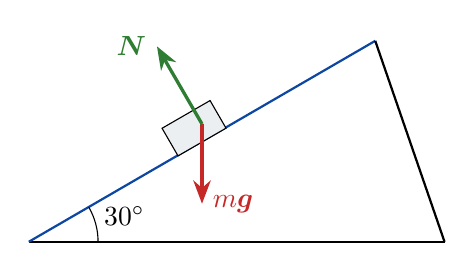
\begin{tikzpicture}[>=Stealth,scale=.88]
\draw[thick] (0,0)--(6,0); \draw[thick,eublue] (0,0)--(5,2.9);
\draw[thick] (5,2.9)--(6,0); \draw[fill=eugrey,rotate around={30:(2.5,1.44)}]
  (2.1,1.44) rectangle (2.9,1.9);
\draw[->,very thick,eured] (2.5,1.7)--(2.5,.55) node[right] {$m\vect g$};
\draw[->,very thick,eugreen] (2.5,1.7)--(1.85,2.82) node[left] {$\vect N$};
\draw (1,0) arc[start angle=0,end angle=30,radius=1];
\node at (1.38,.37) {$30^\circ$};
\end{tikzpicture}
\end{center}

\begin{solucao}[title=Ficha 4]
\textbf{F4.1} $y(t)=-4t+5t^2$ (SI). Subida máxima
$h=v_0^2/(2g)=\SI{0.8}{m}$; distância $0.8+(6+0.8)=\SI{7.6}{m}$.
À altura inicial, rapidez \SI{4}{m.s^{-1}} na descida.\par
\textbf{F4.2} $a=-g\sin30^\circ=-\SI{5}{m.s^{-2}}$;
$0=6^2+2(-5)\Delta x$, logo $\Delta x=\SI{3.6}{m}$.\par
\textbf{F4.3} $GMm/r^2=mv^2/r=m(2\pi r/T)^2/r$;
$T=2\pi\sqrt{r^3/(GM)}$. A razão dos períodos é $2^{3/2}\approx2.83$.
\end{solucao}

\section{Ficha 5 — Mecânica: síntese e queda com ar}
\begin{exercicios}[title=Questões da ficha 5]
\begin{enumerate}[label=F5.\arabic*.]
\item Um balão desce com aceleração instantânea de \SI{4.6}{m.s^{-2}}.
Considera $g=\SI{10}{m.s^{-2}}$ e resistência do ar vertical para cima.
Determina $F_{\mathrm{ar}}/P$.
\item A rapidez de uma esfera aumenta de \SI{0.8}{m.s^{-1}} para
\SI{1.6}{m.s^{-1}} entre $t=\SI{0.5}{s}$ e $t=\SI{1}{s}$.
Determina $a_m$ nesse intervalo, se o movimento ocorre no sentido positivo.
\item Um paraquedas desce a velocidade terminal constante. Compara
intensidade e sentido do peso e da resistência do ar; explica por que
a resultante se anula apesar de a velocidade ser diferente de zero.
\end{enumerate}
\end{exercicios}

\begin{solucao}[title=Ficha 5]
\textbf{F5.1} Tomando para baixo como positivo, $mg-F_{\rm ar}=ma$;
$F_{\rm ar}/P=1-a/g=1-0.46=0.54$.\par
\textbf{F5.2} $a_m=(1.6-0.8)/(1-0.5)=\SI{1.6}{m.s^{-2}}$.\par
\textbf{F5.3} Em regime terminal $F_{\rm ar}=P$ em módulo;
resistência para cima e peso para baixo. A segunda lei impõe
$a=0$, o que significa velocidade constante e não repouso.
\end{solucao}

\part{Física — Ondas e eletromagnetismo}
% =========================================================

\chapter{Sinais, ondas e som}
\begin{objetivos}
\begin{itemize}
  \item distinguir sinal, pulso e onda periódica;
  \item classificar ondas mecânicas/eletromagnéticas e transversais/longitudinais;
  \item relacionar período, frequência, comprimento de onda e velocidade;
  \item interpretar gráficos temporais e espaciais de ondas;
  \item identificar o som como onda de pressão;
  \item analisar sinais sonoros e determinar experimentalmente a velocidade do som.
\end{itemize}
\end{objetivos}

\section{Propagação de uma perturbação}
Uma onda transporta energia e informação sem transporte macroscópico permanente de matéria. Numa onda mecânica, as partículas do meio oscilam em torno das posições de equilíbrio. Ondas eletromagnéticas propagam-se no vazio.

Numa onda transversal, a oscilação é perpendicular à propagação; numa longitudinal, é paralela. O som no ar é uma onda longitudinal de pressão, com compressões e rarefações.

\section{Periodicidade temporal e espacial}
O período $T$ é o tempo de uma oscilação e $f=1/T$. O comprimento de onda $\lambda$ é a distância entre pontos consecutivos em igual fase. A velocidade de propagação é
\[
v=\lambda f.
\]
Ao atravessar uma fronteira, a frequência é imposta pela fonte e não muda; velocidade e comprimento de onda podem mudar.

\begin{center}
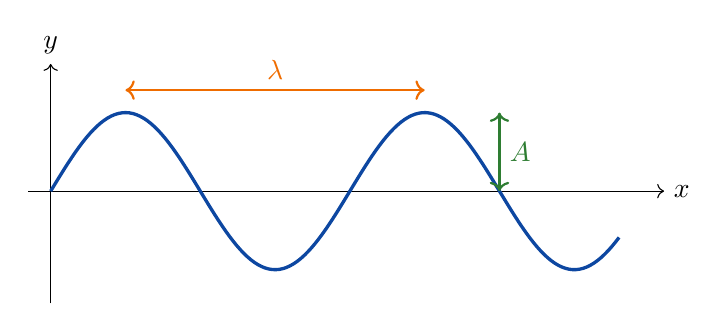
\begin{tikzpicture}[scale=.95]
\draw[->] (-.3,0)--(8.2,0) node[right] {$x$};
\draw[->] (0,-1.5)--(0,1.7) node[above] {$y$};
\draw[eublue,very thick,samples=160,domain=0:7.6] plot (\x,{1.05*sin(90*\x)});
\draw[<->,euorange,thick] (1,1.35)--(5,1.35) node[midway,above] {$\lambda$};
\draw[<->,eugreen,thick] (6,0)--(6,1.05) node[midway,right] {$A$};
\end{tikzpicture}
\end{center}

\begin{exemplo}[title=Exemplo resolvido — frequência e comprimento de onda]
Uma onda sonora de frequência \SI{680}{Hz} propaga-se no ar a \SI{340}{m.s^{-1}}. Então
\[
\lambda=\frac{v}{f}=\frac{340}{680}=\SI{0.50}{m}.
\]
\end{exemplo}

\section{Sinal harmónico}
Um oscilador harmónico pode ser descrito por
\[
y(t)=A\sin(2\pi ft+\varphi),
\]
onde $A$ é amplitude e $\varphi$ fase inicial. Um gráfico $y(t)$ num ponto do espaço revela periodicidade temporal; uma fotografia $y(x)$ num instante revela periodicidade espacial. Confundir estes gráficos leva a atribuir unidades erradas ao eixo horizontal.

\section{Som: frequência, amplitude e forma de onda}
A frequência relaciona-se com a altura percebida; a amplitude de pressão relaciona-se com intensidade, mas a perceção de volume sonoro não é linear. O timbre depende do conteúdo harmónico e da evolução temporal. Sons complexos não são necessariamente ruído; um instrumento musical produz sobreposição organizada de frequências.

\begin{atividade}[title=Características de sinais sonoros]
Liga um microfone a um osciloscópio ou sistema digital. Observa diapasão, voz e instrumento. Mede o período no ecrã e calcula $f$. Compara amplitude, frequência dominante e forma de onda. Mantém a geometria microfone--fonte e o ganho do sistema para comparar amplitudes.

\textbf{Questões:} duplicar a frequência altera o período de que forma? Um som mais intenso altera obrigatoriamente a frequência? Por que a mesma nota pode ter formas de onda diferentes?
\end{atividade}

\begin{atividade}[title=Determinação da velocidade do som]
Coloca dois microfones separados por uma distância $d$ conhecida e produz um pulso perto de um deles. Mede o atraso $\Delta t$ entre sinais e calcula $v=d/\Delta t$. Repetir para várias distâncias e representar $d$ em função de $\Delta t$; o declive estima $v$.

\textbf{Fontes de incerteza:} distância efetiva entre membranas, taxa de amostragem, identificação do início do pulso, reflexões e temperatura. Registar a temperatura do ar e comparar com um valor de referência adequado.
\end{atividade}

\begin{seguranca}
Evitar níveis sonoros elevados, especialmente com auscultadores. A ausência de dor não garante exposição segura; limitar intensidade e duração.
\end{seguranca}

\begin{exercicios}[title=Exercícios do capítulo 10]
\begin{enumerate}[label=10.\arabic*.]
  \item Uma onda tem período \SI{4.0}{ms}. Determina a frequência.
  \item Uma onda de \SI{50}{Hz} propaga-se a \SI{200}{m.s^{-1}}. Calcula $\lambda$.
  \item Uma fonte mantém a frequência ao passar do meio A para B. Se a velocidade diminui \SI{25}{\percent}, como varia $\lambda$?
  \item Num sinal $y(t)$, dois máximos consecutivos ocorrem em \SI{2.4}{ms} e \SI{5.9}{ms}. Determina $T$ e $f$.
  \item Dois microfones separados por \SI{1.70}{m} registam atraso de \SI{5.0}{ms}. Determina a velocidade do som.
  \item Distingue frequência, intensidade e timbre sem usar apenas exemplos musicais.
\end{enumerate}
\end{exercicios}

\section{Aprofundamento — fase, harmónicos e som}
Uma onda periódica num meio pode ser descrita por
\[
y(x,t)=A\sin\!\left(2\pi\frac{t}{T}
             -2\pi\frac{x}{\lambda}+\varphi_0\right).
\]
Dois pontos de uma onda progressiva separados de um múltiplo
inteiro de $\lambda$ oscilam em fase; separados de
$\lambda/2$ têm fases opostas. Para sinais harmónicos,
$\omega=2\pi f=2\pi/T$; num meio homogéneo sem dispersão,
$v=\lambda f$. Ao atravessar uma fronteira entre meios, a
frequência imposta pela fonte mantém-se, enquanto $v$ e
$\lambda$ podem mudar.
\begin{center}
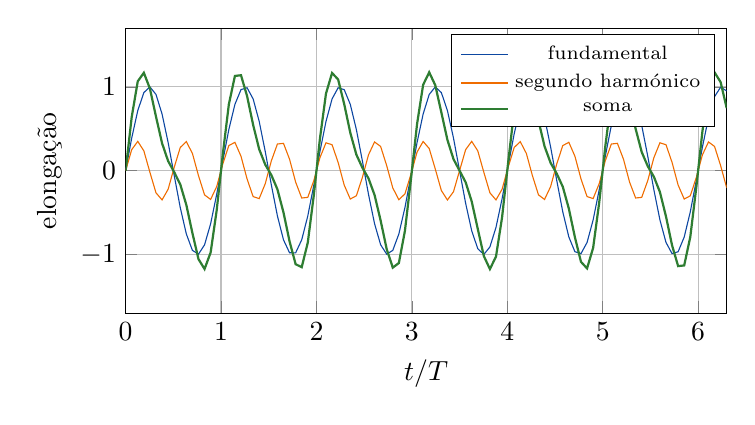
\begin{tikzpicture}
\begin{axis}[width=.76\textwidth,height=5.2cm,xmin=0,xmax=6.3,
ymin=-1.7,ymax=1.7,xlabel={$t/T$},ylabel={elongação},grid=both,
legend style={at={(.98,.98)},anchor=north east,font=\scriptsize}]
\addplot[eublue,domain=0:6.3,samples=100]{sin(deg(2*pi*x))};
\addlegendentry{fundamental}
\addplot[euorange,domain=0:6.3,samples=100]{.35*sin(deg(4*pi*x))};
\addlegendentry{segundo harmónico}
\addplot[eugreen,thick,domain=0:6.3,samples=100]
  {sin(deg(2*pi*x))+.35*sin(deg(4*pi*x))};
\addlegendentry{soma}
\end{axis}
\end{tikzpicture}
\end{center}
No gráfico, a curva verde é a soma matemática das outras duas;
serve para visualizar por que um som complexo pode ter forma
distinta da sinusoidal mesmo com uma periodicidade reconhecível.
\begin{nota}
A \emph{altura} relaciona-se com a frequência e permite distinguir
sons graves de agudos. A \emph{intensidade} e a sensação de volume
relacionam-se com energia/amplitude e também com a resposta do
ouvido. O \emph{timbre} depende do conteúdo espectral e da evolução
temporal. No resumo de origem, a palavra «altura» surgia também
associada à amplitude; aqui emprega-se «intensidade» nesse caso.
\end{nota}
\begin{atividade}[title=Do diapasão ao espetro sonoro]
Grava dois instrumentos a tocar a mesma nota, com volume moderado.
Examina a forma de onda e o espetro de frequências; identifica a
fundamental e os harmónicos. Compara os timbres sem interpretar
a altura das barras espectrais como energia absoluta sem calibrar
o microfone. Regista a taxa de amostragem e discute ruído ambiente.
\end{atividade}


\section{Sinais, instantâneos espaciais e som}
Um sinal é uma perturbação local que pode transportar informação.
Uma perturbação de curta duração origina um pulso; uma fonte
periódica pode criar uma onda periódica. A onda transfere energia
sem transporte macroscópico permanente da matéria do meio.
\begin{table}[H]
\centering\small
\caption{Duas formas de classificar as ondas.}
\begin{tabularx}{\textwidth}{@{}p{.22\textwidth}p{.32\textwidth}X@{}}
\toprule
Critério & Classe & Exemplo e propriedade\\\midrule
Natureza & mecânica & som no ar; exige meio material\\
Natureza & eletromagnética & rádio e luz; propaga-se no vazio\\
Vibração & transversal & oscilação perpendicular ao avanço\\
Vibração & longitudinal & oscilação paralela ao avanço,
como a compressão do ar numa onda sonora\\
\bottomrule\end{tabularx}
\end{table}
Num gráfico $y(t)$ de um único ponto, a separação temporal entre
máximos sucessivos é o período $T$, em segundos.
Num gráfico $y(x)$ de vários pontos no mesmo instante,
a separação espacial entre máximos sucessivos é
$\lambda$, em metros. A amplitude $A$ é o afastamento
máximo da posição de equilíbrio. É incorreto ler
$\lambda$ numa escala temporal ou $T$ numa escala espacial.
\begin{center}
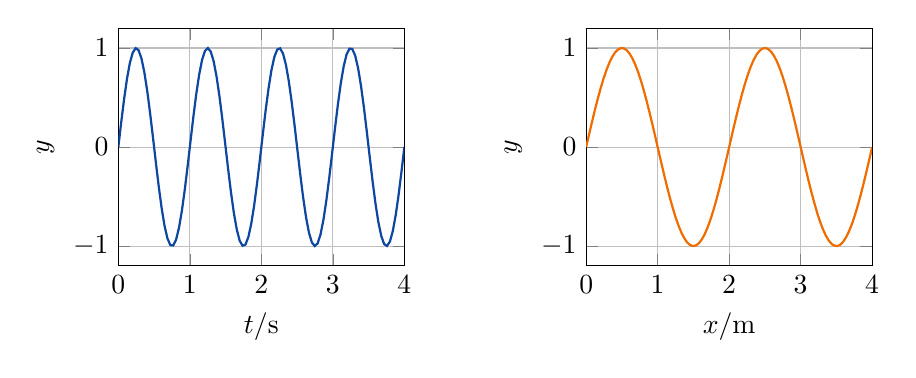
\begin{tikzpicture}
\begin{axis}[at={(0,0)},anchor=south west,width=.43\textwidth,
height=4.6cm,xmin=0,xmax=4,ymin=-1.2,ymax=1.2,
xlabel={$t$/s},ylabel={$y$},xtick={0,1,2,3,4},
ytick={-1,0,1},grid=major]
\addplot[eublue,thick,domain=0:4,samples=100] {sin(deg(2*pi*x))};
\end{axis}
\begin{axis}[at={(.49\textwidth,0)},anchor=south west,
width=.43\textwidth,height=4.6cm,xmin=0,xmax=4,
ymin=-1.2,ymax=1.2,xlabel={$x$/m},ylabel={$y$},
xtick={0,1,2,3,4},ytick={-1,0,1},grid=major]
\addplot[euorange,thick,domain=0:4,samples=100] {sin(deg(pi*x))};
\end{axis}
\end{tikzpicture}
\end{center}
Os gráficos ilustram $T=\SI{1}{s}$ e
$\lambda=\SI{2}{m}$. Se representarem a mesma onda num
meio uniforme, $v=\lambda/T=\SI{2}{m.s^{-1}}$.
Pontos separados por $\lambda$ estão em fase; pontos
separados por $\lambda/2$ vibram em oposição de fase.
\begin{exemplo}[title=Exemplo resolvido — mudança de meio]
Uma fonte produz som de frequência \SI{250}{Hz}. Com
$v_1=\SI{340}{m.s^{-1}}$, $\lambda_1=340/250
=\SI{1.36}{m}$. Num segundo meio, se
$v_2=\SI{680}{m.s^{-1}}$, a frequência e o período
mantêm-se e $\lambda_2=\SI{2.72}{m}$.
\end{exemplo}
No ar, o som é uma onda mecânica longitudinal de
compressões e rarefações. Para um som harmónico,
a perturbação de pressão num ponto pode escrever-se
$p(t)=p_{\max}\sin(\omega t+\varphi)$, com
$\omega=2\pi f$. A frequência está ligada à
altura percebida (grave ou agudo); a amplitude
da pressão contribui para a intensidade; a forma
de onda e os harmónicos contribuem para o timbre.
O som não se propaga no vácuo.

Um microfone transforma variações de pressão sonora
em sinal elétrico; um altifalante realiza a
conversão inversa. Num microfone dinâmico, o
movimento relativo entre bobina e íman induz uma
tensão. No altifalante, uma corrente variável na
bobina move um cone, que perturba o ar.


\section{Ficha 6 — Sinais, ondas e som}
\begin{exercicios}[title=Questões da ficha 6]
\begin{enumerate}[label=F6.\arabic*.]
\item Uma extremidade de uma corda é perturbada durante \SI{20}{ms},
gerando um pulso que se propaga a \SI{12}{m.s^{-1}}. Calcula a largura
espacial do pulso e os instantes de início e fim da perturbação num ponto
a \SI{2}{m} da fonte.
\item Uma onda periódica na mesma corda tem frequência de \SI{40}{Hz}.
Determina período e comprimento de onda. Se a frequência passar a
\SI{80}{Hz}, mantendo-se as condições da corda, que sucede à velocidade
e ao comprimento de onda?
\item Explica por que uma onda longitudinal numa mola não modela a
polarização da luz; indica uma diferença entre ondas mecânicas e
eletromagnéticas quanto ao meio de propagação.
\end{enumerate}
\end{exercicios}

\begin{solucao}[title=Ficha 6]
\textbf{F6.1} Largura $v\Delta t=12(0.020)=\SI{0.24}{m}$.
Chegada da frente: $2/12=\SI{0.167}{s}$; passagem da cauda:
$0.167+0.020=\SI{0.187}{s}$.\par
\textbf{F6.2} $T=1/f=\SI{0.025}{s}$;
$\lambda=v/f=12/40=\SI{0.30}{m}$.
A nova frequência conserva $v$ e reduz $\lambda$ a \SI{0.15}{m}.\par
\textbf{F6.3} Numa onda longitudinal, deslocamento e propagação são
paralelos; a polarização de luz diz respeito à direção transversal do
campo elétrico. A onda da mola precisa de matéria; a luz propaga-se
também no vácuo.
\end{solucao}

\chapter{Campos elétricos, campos magnéticos e indução}
\begin{objetivos}
\begin{itemize}
  \item identificar fontes de campos elétricos e magnéticos;
  \item interpretar linhas de campo e forças sobre cargas/ímanes;
  \item reconhecer os contributos de Oersted, Faraday, Maxwell e Hertz;
  \item relacionar variação do fluxo magnético e força eletromotriz induzida;
  \item explicar geradores, transformadores e aplicações da indução.
\end{itemize}
\end{objetivos}

\section{Campo como modelo físico}
Um campo atribui a cada ponto do espaço uma grandeza. Cargas elétricas originam campo elétrico; correntes elétricas e ímanes originam campo magnético. Linhas de campo são representações: a tangente indica direção, a densidade sugere intensidade e as linhas não são objetos materiais.

Para uma carga de prova positiva $q$,
\[
\vect F_e=q\vect E.
\]
Uma carga negativa sofre força oposta ao campo. Um íman num campo magnético tende a orientar-se, evidenciando direção e sentido convencional do campo.

\begin{center}

\begin{tikzpicture}[>=Stealth,scale=.9]
\fill[eured] (-2.6,0) circle (.28) node[white] {$+$};
\foreach \a in {0,45,...,315}{\draw[->,eured,thick] (-2.6,0)--++(\a:1.45);}
\fill[eublue] (2.6,0) circle (.28) node[white] {$-$};
\foreach \a in {0,45,...,315}{\draw[->,eublue,thick] ($(2.6,0)+(\a:1.45)$)--(2.6,0);}
\end{tikzpicture}
\end{center}

\section{Da eletricidade ao eletromagnetismo}
Oersted mostrou que uma corrente desvia uma bússola, ligando eletricidade e magnetismo. Faraday descobriu a indução eletromagnética. Maxwell sintetizou eletricidade, magnetismo e ótica numa teoria que previa ondas eletromagnéticas. Hertz produziu e detetou essas ondas experimentalmente. Esta sequência ilustra a ciência como construção coletiva: experiência, modelo matemático, previsão e teste.

\section{Fluxo magnético e Lei de Faraday}
Para campo uniforme e uma espira plana,
\[
\Phi=B A\cos\theta,
\]
onde $\theta$ é o ângulo entre $\vect B$ e a normal ao plano. A força eletromotriz induzida média numa bobina de $N$ espiras é
\[
|\mathcal E|=N\frac{|\Delta\Phi|}{\Delta t}.
\]
O sentido da corrente induzida opõe-se à variação do fluxo que a originou (Lei de Lenz), expressão da conservação da energia.

\begin{exemplo}[title=Exemplo resolvido — fem induzida]
Uma bobina de 200 espiras, área \SI{3.0e-3}{m^2}, está perpendicular a um campo que varia de \SI{0.10}{T} para \SI{0.40}{T} em \SI{0.050}{s}. Com $\cos\theta=1$,
\[
|\mathcal E|=200\frac{3,0\times10^{-3}(0,40-0,10)}{0,050}=\SI{3.6}{V}.
\]
\end{exemplo}

\section{Como variar o fluxo}
Pode induzir-se uma fem variando a intensidade de $B$, a área da espira, a orientação ou deslocando a bobina entre regiões de campo diferente. “Existir campo” não basta: é necessária variação do fluxo através do circuito.

\begin{atividade}[title=Linhas de campo e indução]
\textbf{Parte A:} mapear qualitativamente o campo de um íman com pequenas bússolas ou limalha protegida por uma folha/recipiente selado. Comparar com o campo em torno de um condutor/bobina atravessado por corrente baixa.

\textbf{Parte B:} ligar uma bobina a um galvanómetro/sensor e mover um íman. Testar rapidez, sentido, número de espiras e imobilidade. Registar sinal e máximo da fem. Concluir que uma variação mais rápida do fluxo produz maior $|\mathcal E|$.
\end{atividade}

\begin{seguranca}
Usar fontes de baixa tensão e limitar a corrente. Não ligar bobinas diretamente à rede. Ímanes fortes devem ficar longe de dispositivos médicos, cartões e objetos que possam ser projetados.
\end{seguranca}

\section{Geradores e transformadores}
Num gerador, energia mecânica faz variar o fluxo e produz corrente elétrica. Num transformador ideal de corrente alternada,
\[
\frac{V_s}{V_p}=\frac{N_s}{N_p},\qquad V_pI_p\approx V_sI_s.
\]
Elevar a tensão no transporte reduz a corrente para a mesma potência e diminui perdas por efeito Joule, $P_{perdas}=RI^2$.

\begin{mundo}
Indução está presente em centrais elétricas, carregamento sem fios, travagem magnética, placas de indução, microfones dinâmicos e sensores. Em cada aplicação há conversão de energia e compromisso entre eficiência, materiais, custo e segurança.
\end{mundo}

\begin{exercicios}[title=Exercícios do capítulo 11]
\begin{enumerate}[label=11.\arabic*.]
  \item Uma carga positiva de \SI{2.0}{\micro C} está num campo de \SI{3.0e4}{N.C^{-1}}. Calcula a força elétrica.
  \item Explica o que significa maior densidade de linhas num diagrama de campo.
  \item Uma espira de área \SI{0.020}{m^2} está perpendicular a $B=\SI{0.15}{T}$. Calcula o fluxo.
  \item Numa bobina de 500 espiras, o fluxo por espira varia \SI{2.0e-4}{Wb} em \SI{0.10}{s}. Calcula a fem média.
  \item Explica por que um íman imóvel dentro de uma bobina não mantém corrente induzida.
  \item Um transformador tem 1000 espiras no primário e 100 no secundário. Se $V_p=\SI{230}{V}$, determina $V_s$ no modelo ideal.
\end{enumerate}
\end{exercicios}

\section{Aprofundamento — campos e indução}
Uma carga positiva cria um campo elétrico radial para fora, e
uma carga negativa cria-o radial para dentro. Em cada ponto,
$\vect E$ é tangente à linha de campo. As linhas são uma
convenção de desenho: a sua densidade representa qualitativamente
a intensidade, sem corresponder a uma quantidade física de linhas.
\begin{center}
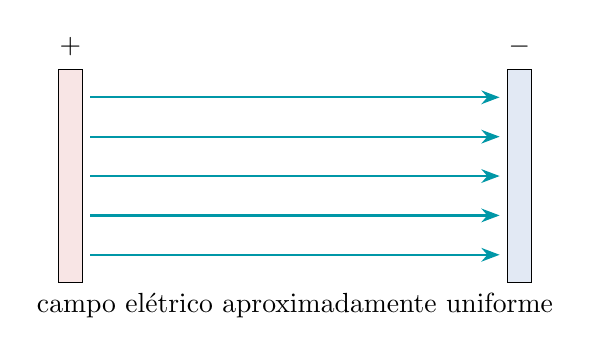
\begin{tikzpicture}[>=Stealth]
\draw[fill=eured!12] (-3,-1.35) rectangle (-2.7,1.35);
\draw[fill=eublue!12] (2.7,-1.35) rectangle (3,1.35);
\node at (-2.85,1.65) {$+$}; \node at (2.85,1.65) {$-$};
\foreach \yy in {-1,-.5,0,.5,1}
  \draw[->,eucyan,thick] (-2.6,\yy)--(2.6,\yy);
\node at (0,-1.65) {campo elétrico aproximadamente uniforme};
\end{tikzpicture}
\end{center}
O campo magnético de um fio retilíneo percorrido por corrente
apresenta linhas circulares centradas no fio. O sentido segue a
regra da mão direita. No interior de um solenoide comprido, longe
das extremidades, o campo pode ser aproximadamente uniforme.
\begin{exemplo}[title=Exemplo resolvido — orientação e fluxo]
Uma espira de área \SI{0.020}{m^2} está num campo uniforme
$B=\SI{0.15}{T}$. Se a normal à espira fizer $60^\circ$ com
$\vect B$, o fluxo é $\Phi=BA\cos60^\circ
=\SI{1.5e-3}{Wb}$. É máximo com a normal paralela a $\vect B$,
e nulo com a normal perpendicular a $\vect B$.
\end{exemplo}
\begin{metodo}[title=Como aplicar a lei de Faraday--Lenz]
\begin{enumerate}
\item Identifica a área, a orientação da normal e o campo magnético.
\item Calcula o fluxo por espira $\Phi=BA\cos\alpha$ e a sua variação.
\item Calcula o módulo $|\mathcal E|=N|\Delta\Phi|/\Delta t$.
\item Usa a lei de Lenz para decidir o sentido do campo criado
pela corrente induzida. Só depois aplica a regra da mão direita
para determinar o sentido da corrente na espira.
\end{enumerate}
\end{metodo}
\begin{stem}
Projeta um gerador manual com bobina, íman e LED. Conta as espiras,
mede qualitativamente a tensão induzida com diferentes velocidades
de rotação e documenta que grandezas foram mantidas constantes.
Explica por que um íman imóvel relativamente à bobina pode produzir
campo sem induzir uma força eletromotriz permanente.
\end{stem}


\section{Cargas, campos e aplicações da indução}
Num sistema isolado, a carga elétrica total conserva-se.
Em processos de fricção, eletrões podem transferir-se
entre objetos; os protões mantêm-se nos núcleos.
Um corpo positivo tem défice de eletrões
relativamente ao seu estado neutro. A carga
é quantizada: $Q=ne$, com $n$ inteiro e
$e\simeq\SI{1.602e-19}{C}$.
\begin{center}
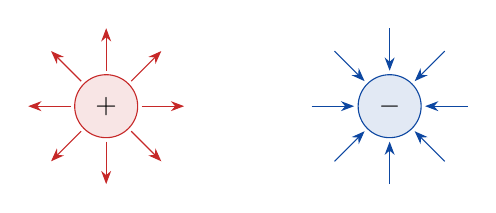
\begin{tikzpicture}[>=Stealth,scale=.9]
\node[circle,draw=eured,fill=eured!12,minimum size=8mm]
 (p) at (-2,0) {$+$};
\node[circle,draw=eublue,fill=eublue!12,minimum size=8mm]
 (m) at (2,0) {$-$};
\foreach \a in {0,45,90,135,180,225,270,315}{
 \draw[->,eured] ($(p)+(\a:.5)$)--($(p)+(\a:1.1)$);
 \draw[->,eublue] ($(m)+(\a:1.1)$)--($(m)+(\a:.5)$);
}
\end{tikzpicture}
\end{center}
As setas mostram o sentido do campo de cada carga
isolada. Quando as duas cargas estão presentes, o
campo em cada ponto é a soma vetorial dos campos,
e as linhas do campo conjunto devem ser
desenhadas a partir dessa soma.
Para uma carga de prova, $\vect F_e=q\vect E$.
Se $q<0$, a força tem sentido contrário a $\vect E$.

Uma bússola orienta-se segundo o campo magnético
local. Perto de um fio longo percorrido por corrente,
as linhas de $\vect B$ são circunferências centradas
no fio, em planos perpendiculares a ele. Com o polegar
da mão direita no sentido da corrente convencional,
os dedos curvados indicam o sentido das linhas.
Num solenoide comprido, o campo interior é
aproximadamente uniforme longe das extremidades.
\begin{nota}
As linhas do campo magnético são fechadas: no exterior
de um íman dirigem-se do polo norte para o sul; no
interior, regressam do sul ao norte. A densidade das
linhas desenhadas indica qualitativamente a
intensidade do campo, cuja unidade é o tesla.
\end{nota}

Para uma espira plana de área $A$ num campo
uniforme, $\Phi=BA\cos\alpha$, sendo $\alpha$
o ângulo entre $\vect B$ e a normal à espira.
Se o fluxo por espira variar, numa bobina de $N$
espiras a fem induzida média tem módulo
$|\mathcal E|=N|\Delta\Phi|/\Delta t$.
\begin{table}[H]
\centering\small
\caption{Três orientações da espira relativamente ao campo.}
\begin{tabular}{@{}ccc@{}}\toprule
$\alpha$ & $\Phi/(BA)$ & Interpretação\\\midrule
$0^\circ$ & $+1$ & fluxo positivo máximo\\
$90^\circ$ & $0$ & sem componente normal do campo\\
$180^\circ$ & $-1$ & fluxo negativo máximo\\
\bottomrule\end{tabular}
\end{table}
Uma espira imóvel num campo estático pode ter fluxo
não nulo sem fem induzida: é a variação do fluxo que
importa. Se o circuito estiver aberto pode existir
tensão induzida, mas não corrente sustentada através
da abertura. O sentido de uma corrente induzida
num circuito fechado segue a lei de Lenz.

\section{Ficha 7 — Campo elétrico, campo magnético e indução}
\begin{exercicios}[title=Questões da ficha 7]
\begin{enumerate}[label=F7.\arabic*.]
\item Uma barra inicialmente neutra fica positivamente carregada por
fricção. Que partículas foram transferidas e em que sentido? Explica
por que a conservação da carga não exige que a barra permaneça neutra.
\item Uma carga $q=-\SI{2.0}{\micro C}$ está num campo uniforme
$\vect E$ dirigido para a direita, de módulo \SI{3.0e4}{N.C^{-1}}.
Determina a força e representa o seu sentido.
\item Uma bobina de 200 espiras sofre diminuição uniforme do fluxo por
espira de $\SI{5e-3}{Wb}$ para $\SI{1e-3}{Wb}$ em \SI{0.20}{s}.
Calcula o módulo da força eletromotriz induzida e enuncia como se
determina o sentido da corrente induzida.
\end{enumerate}
\end{exercicios}

\begin{solucao}[title=Ficha 7]
\textbf{F7.1} Eletrões saíram da barra para o outro material; a
carga total do sistema isolado conserva-se pela transferência.\par
\textbf{F7.2} $|F|=|q|E=(2.0\times10^{-6})(3.0\times10^4)
=\SI{0.060}{N}$. Por $q<0$, a força aponta para a esquerda.\par
\textbf{F7.3} $|\mathcal E|=N|\Delta\Phi|/\Delta t
=200(0.004)/0.20=\SI{4.0}{V}$. O sentido segue a lei de Lenz:
a corrente cria um campo que se opõe à diminuição do fluxo.
\end{solucao}

\chapter{Ondas eletromagnéticas, luz e comunicações}
\begin{objetivos}
\begin{itemize}
  \item caracterizar o espetro eletromagnético e relacionar $c$, $f$ e $\lambda$;
  \item aplicar as leis da reflexão e da refração;
  \item interpretar reflexão total e fibras óticas;
  \item reconhecer difração como fenómeno ondulatório;
  \item determinar experimentalmente índice de refração e comprimento de onda;
  \item fundamentar aplicações em comunicações e no estudo do Universo.
\end{itemize}
\end{objetivos}

\section{Espetro eletromagnético}
Todas as ondas eletromagnéticas se propagam no vazio a $c\approx\SI{3.00e8}{m.s^{-1}}$ e satisfazem $c=\lambda f$. Rádio, micro-ondas, infravermelho, visível, ultravioleta, raios X e gama diferem em frequência/comprimento de onda e na forma como interagem com a matéria. “Radiação” não significa automaticamente “ionizante” ou “perigosa”; risco depende de frequência, intensidade, duração e interação biológica.

\begin{exemplo}[title=Exemplo resolvido — onda de rádio]
Para $f=\SI{100}{MHz}=1,00\times10^8\ \si{Hz}$,
\[
\lambda=\frac{c}{f}=\frac{3,00\times10^8}{1,00\times10^8}=\SI{3.00}{m}.
\]
\end{exemplo}

\section{Reflexão}
Os ângulos medem-se relativamente à normal:
\[
\theta_i=\theta_r.
\]
Reflexão especular ocorre em superfícies lisas à escala do comprimento de onda; superfícies rugosas originam reflexão difusa, ainda obedecendo localmente à lei.

\section{Refração e índice de refração}
O índice é $n=c/v$. Na passagem entre meios,
\[
n_1\sin\theta_1=n_2\sin\theta_2.
\]
Ao entrar num meio de maior índice, a luz aproxima-se da normal. A frequência não muda; a velocidade e o comprimento de onda diminuem.

\begin{center}
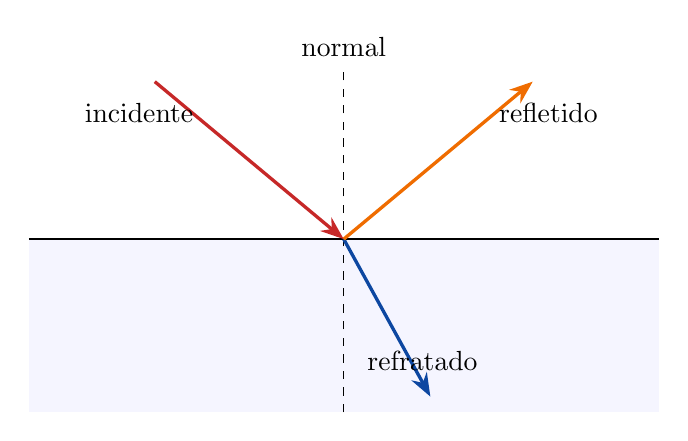
\begin{tikzpicture}[>=Stealth,scale=1.0]
\fill[blue!4] (-4,-2.2) rectangle (4,0);
\draw[thick] (-4,0)--(4,0);
\draw[dashed] (0,-2.2)--(0,2.2) node[above] {normal};
\draw[eured,very thick,->] (-2.4,2)--(0,0);
\draw[eublue,very thick,->] (0,0)--(1.1,-2);
\draw[euorange,very thick,->] (0,0)--(2.4,2);
\node at (-2.6,1.6) {incidente};
\node at (1.0,-1.55) {refratado};
\node at (2.6,1.6) {refletido};
\end{tikzpicture}
\end{center}

\begin{exemplo}[title=Exemplo resolvido — Lei de Snell]
Luz passa do ar ($n_1=1,00$) para vidro ($n_2=1,50$) com $\theta_1=30,0^\circ$. Então
\[
\sin\theta_2=\frac{1,00}{1,50}\sin30,0^\circ=0,333,
\]
e $\theta_2\approx19,5^\circ$.
\end{exemplo}

\section{Reflexão total}
Ao passar de maior para menor índice, existe um ângulo crítico $\theta_c$:
\[
\sin\theta_c=\frac{n_2}{n_1}\quad(n_1>n_2).
\]
Para incidência superior a $\theta_c$, ocorre reflexão total. Fibras óticas guiam luz por este fenómeno, embora perdas, dispersão e curvatura imponham limites.

\section{Difração e medição de \texorpdfstring{$\lambda$}{lambda}}
Ondas contornam obstáculos e espalham-se em aberturas, sobretudo quando as dimensões são comparáveis a $\lambda$. Numa rede de difração,
\[
d\sin\theta=m\lambda,
\]
onde $d$ é o espaçamento entre linhas e $m$ a ordem do máximo.

\begin{atividade}[title=Índice de refração de um material]
Faz incidir um feixe laser num bloco semicircular ou placa transparente. Mede vários pares $(\theta_1,\theta_2)$ relativamente à normal. Representa $\sin\theta_1$ em função de $\sin\theta_2$. Se o primeiro meio for ar, o declive estima $n_2$.

\textbf{Avaliação:} largura do feixe, espessura dos traços, alinhamento, centro geométrico, leitura angular e escolha do ajuste.
\end{atividade}

\begin{atividade}[title=Comprimento de onda de um laser]
Incide um laser numa rede de difração de espaçamento conhecido $d$. A uma distância $L$, mede a distância $y_m$ do máximo central ao máximo de ordem $m$. Determina $\theta$ por $\tan\theta=y_m/L$ e calcula $\lambda=d\sin\theta/m$. Mede de ambos os lados e faz média para reduzir erro de alinhamento.
\end{atividade}

\begin{seguranca}
Nunca dirigir laser para olhos, pessoas, veículos ou superfícies muito refletoras. Usar apenas lasers escolares de baixa potência e manter o feixe abaixo do nível dos olhos, terminado num alvo opaco.
\end{seguranca}

\section{Comunicações e conhecimento do Universo}
As telecomunicações escolhem bandas segundo alcance, largura de banda, absorção, antenas, interferência e regulamentação. A astronomia multimensageira combina rádio, infravermelho, visível, ultravioleta, raios X, gama, partículas e ondas gravitacionais. Cada janela revela processos diferentes; modelos científicos são revistos quando novos instrumentos produzem evidência incompatível com previsões anteriores.

\begin{stem}
\textbf{Rede de comunicações de emergência.} Concebe uma solução para uma comunidade isolada após um evento extremo. Compara rádio, micro-ondas, fibra e satélite em alcance, energia, atraso, capacidade, robustez, custo e manutenção. Produz uma recomendação sustentada, incluindo limitações e plano de redundância.
\end{stem}

\begin{exercicios}[title=Exercícios do capítulo 12]
\begin{enumerate}[label=12.\arabic*.]
  \item Calcula a frequência de luz com $\lambda=\SI{600}{nm}$ no vazio.
  \item Luz passa de vidro $n=1,50$ para ar. Calcula o ângulo crítico.
  \item Um raio incide do ar em água ($n=1,33$) a $45,0^\circ$. Calcula o ângulo refratado.
  \item Num meio com $n=1,60$, determina a velocidade da luz e o comprimento de onda de radiação cuja frequência é \SI{5.0e14}{Hz}.
  \item Uma rede tem 600 linhas por milímetro. O máximo de primeira ordem ocorre a $20,0^\circ$. Calcula $\lambda$.
  \item Explica por que ondas de rádio e raios X são ambos ondas eletromagnéticas, mas têm interações biológicas muito diferentes.
\end{enumerate}
\end{exercicios}

% =========================================================
\section{Aprofundamento — ótica, difração e comunicações}
Na passagem de um feixe de um meio para outro, $f$ mantém-se.
Para dois meios transparentes,
\[
n_1\sin\theta_1=n_2\sin\theta_2,\qquad
v=\frac{c}{n},\qquad \lambda=\frac{v}{f}.
\]
Os ângulos são sempre medidos relativamente à normal à superfície.
\begin{center}
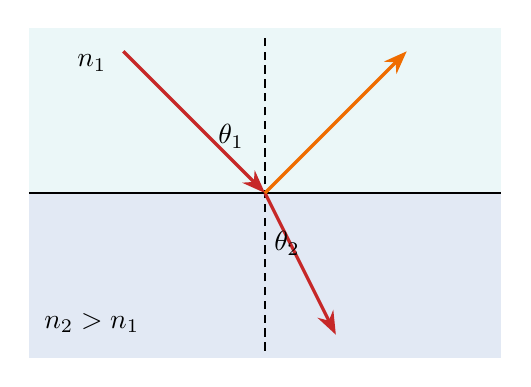
\begin{tikzpicture}[>=Stealth]
\fill[eucyan!8] (-3,0) rectangle (3,2.1);
\fill[eublue!12] (-3,-2.1) rectangle (3,0);
\draw[thick] (-3,0)--(3,0);
\draw[densely dashed] (0,-2)--(0,2);
\draw[->,very thick,eured] (-1.8,1.8)--(0,0);
\draw[->,very thick,eured] (0,0)--(.9,-1.8);
\draw[->,very thick,euorange] (0,0)--(1.8,1.8);
\node at (-2.2,1.65) {$n_1$};
\node at (-2.2,-1.65) {$n_2>n_1$};
\node at (-.43,.72) {$\theta_1$};
\node at (.28,-.64) {$\theta_2$};
\end{tikzpicture}
\end{center}
A reflexão total exige incidência do meio com maior $n$ para
outro com menor $n$ e ângulo acima do crítico
$\theta_c=\arcsin(n_2/n_1)$. Este princípio está na base
do guiamento de luz em fibras óticas. A difração torna-se
mais visível quando a dimensão de uma abertura é comparável
ao comprimento de onda; com uma rede de difração,
$d\sin\theta=m\lambda$ para máximos principais em condições
de incidência normal.
\begin{atividade}[title=Determinar o comprimento de onda com uma rede]
Usa laser de baixa potência adequado ao laboratório, rede de
difração e ecrã. Mede distância rede--ecrã $L$ e deslocamento
horizontal $y$ do máximo de ordem $m=1$. Calcula
$\theta=\arctan(y/L)$ e $\lambda=d\sin\theta$.
Repete medidas, estima a dispersão e mantém o feixe afastado dos olhos.
\end{atividade}
\begin{mundo}
Escolhe entre comunicação por fibra, rádio e som subaquático
para transmitir informação num túnel, no mar e entre satélites.
Justifica a escolha em função da atenuação no meio, da velocidade
de propagação, da infraestrutura e da largura de banda necessária.
\end{mundo}

\section{Luz numa interface: energia e direção dos raios}
Ao chegar à fronteira entre meios, parte da energia
da radiação pode ser refletida, outra parte transmitida
e outra absorvida. Num balanço sem outras saídas,
\[
E_{\rm inc}=E_{\rm refl}+E_{\rm trans}+E_{\rm abs}.
\]
As frações dependem dos meios, da frequência e do
ângulo de incidência. Albedo é uma medida da fração
de radiação incidente refletida por uma superfície
ou sistema numa determinada definição espectral
e geométrica; não se aplica automaticamente
um valor único a qualquer situação.

Na reflexão especular, o raio incidente, a
normal e o raio refletido encontram-se no
mesmo plano e $\theta_i=\theta_r$. Como a
onda permanece no mesmo meio, a frequência,
a velocidade e o comprimento de onda mantêm-se;
a amplitude refletida pode ser diferente.
Numa superfície irregular, a reflexão pode ser
difusa em muitas direções.
\begin{center}
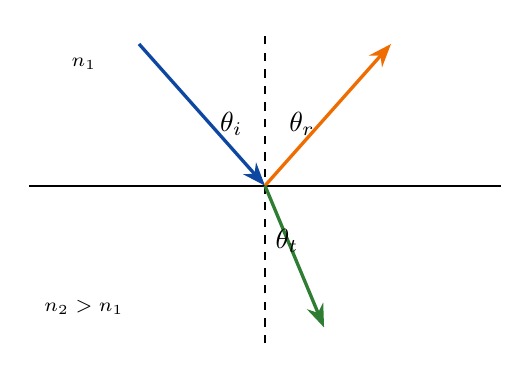
\begin{tikzpicture}[>=Stealth]
\draw[thick] (-3,0)--(3,0);
\draw[dashed] (0,-2)--(0,2);
\draw[->,very thick,eublue] (-1.6,1.8)--(0,0);
\draw[->,very thick,euorange] (0,0)--(1.6,1.8);
\draw[->,very thick,eugreen] (0,0)--(.75,-1.8);
\node at (-.43,.78) {$\theta_i$};
\node at (.47,.78) {$\theta_r$};
\node at (.28,-.7) {$\theta_t$};
\node[font=\scriptsize] at (-2.3,1.55) {$n_1$};
\node[font=\scriptsize] at (-2.3,-1.55) {$n_2>n_1$};
\end{tikzpicture}
\end{center}
Na refração, $n=c/v$ e
$n_1\sin\theta_1=n_2\sin\theta_2$.
Os ângulos são medidos em relação à normal.
Se $n_2>n_1$, o raio aproxima-se da normal,
a velocidade e o comprimento de onda diminuem,
e a frequência mantém-se. Para a mesma
radiação monocromática,
\[
\frac{n_1}{n_2}
=\frac{v_2}{v_1}
=\frac{\lambda_2}{\lambda_1}.
\]
Em meios dispersivos o índice depende da
frequência, pelo que cores diferentes podem
ser desviadas por ângulos distintos.
\begin{exemplo}[title=Exemplo resolvido — balanço e refração]
Um feixe com energia \SI{2.00}{mJ} incide numa
interface: \SI{0.30}{mJ} são refletidos e
\SI{0.20}{mJ} são absorvidos. A energia
transmitida é $2,00-0,30-0,20=\SI{1.50}{mJ}$.
Se $n_1=1,00$, $n_2=1,50$ e
$\theta_1=30^\circ$, então
$\sin\theta_2=\sin30^\circ/1,50=1/3$;
logo $\theta_2\simeq19,5^\circ$.
\end{exemplo}

\section{Reflexão total, fibras e difração}
A reflexão total exige propagação a partir
do meio de maior índice para outro de menor
índice e um ângulo de incidência superior a
$\theta_c=\arcsin(n_2/n_1)$. No modelo de
ótica geométrica deixa de existir raio
transmitido propagante para
$\theta_i>\theta_c$. Perto da interface
pode existir um campo evanescente.
O núcleo de uma fibra ótica é escolhido
em conjunto com um revestimento de índice
inferior, considerando também as perdas
e a faixa de frequências utilizada.

A difração ocorre quando uma onda passa
por uma abertura ou contorna um obstáculo.
É mais evidente quando a dimensão da
abertura é da ordem do comprimento de onda.
Para a mesma onda, uma fenda mais larga
gera espalhamento angular menor do que
uma fenda mais estreita.
\begin{center}
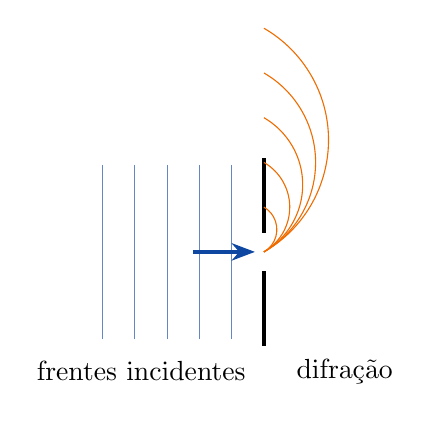
\begin{tikzpicture}[>=Stealth,scale=.82]
\foreach \x in {-2.5,-2,-1.5,-1,-.5}
  \draw[eublue!65] (\x,-1.35)--(\x,1.35);
\draw[very thick] (0,-1.45)--(0,-.3);
\draw[very thick] (0,.3)--(0,1.45);
\foreach \r in {.4,.8,1.2,1.6,2}
  \draw[euorange] (0,0) arc[start angle=-60,end angle=60,radius=\r];
\draw[->,eublue,very thick] (-1.1,0)--(-.14,0);
\node at (-1.9,-1.85) {frentes incidentes};
\node at (1.25,-1.85) {difração};
\end{tikzpicture}
\end{center}
Numa rede de difração com incidência normal,
os máximos principais obedecem a
$d\sin\theta=m\lambda$, quando as condições
geométricas estão satisfeitas.
\begin{stem}
Numa simulação, compara duas larguras de
fenda e dois comprimentos de onda.
Estima a largura angular do máximo central
e regista qual variável se manteve constante
em cada comparação. Relaciona o resultado
com a resolução de um instrumento ótico.
\end{stem}

\section{Da indução às ondas eletromagnéticas}
O estudo histórico de correntes e campos
conduziu à previsão de ondas eletromagnéticas.
Numa onda ideal no vazio, os campos elétrico
e magnético variam no tempo e são
perpendiculares entre si e à direção de
propagação. A luz, as ondas de rádio e as
micro-ondas pertencem ao mesmo espetro;
diferem em frequência e comprimento de onda.
O som é uma perturbação mecânica e, ao
contrário da luz, precisa de um meio material.

Em comunicações, as características do meio
determinam perdas e possibilidades de
transmissão: a fibra guia luz; antenas emitem
e recebem ondas eletromagnéticas; no mar,
o som pode ser utilizado para comunicar
e detetar objetos. Indica sempre o meio
e a distância antes de comparar tecnologias.

\section{Ficha 8 — Luz e ondas eletromagnéticas}
\begin{exercicios}[title=Questões da ficha 8]
\begin{enumerate}[label=F8.\arabic*.]
\item Um feixe monocromático passa do ar para acrílico de índice
$n=1.50$ com ângulo de incidência de $30^\circ$. Determina o ângulo
de refração. Indica o que muda na frequência, velocidade e comprimento
de onda.
\item Calcula o ângulo crítico para luz que passa do acrílico
($n=1.50$) para o ar ($n=1.00$). Explica o requisito para haver
reflexão total.
\item Uma luz de \SI{600}{nm} no vácuo atravessa um material de
$n=1.50$. Usando $c=\SI{3.00e8}{m.s^{-1}}$, calcula $f$, velocidade
e comprimento de onda no material.
\end{enumerate}
\end{exercicios}

\begin{solucao}[title=Ficha 8]
\textbf{F8.1} $\sin\theta_2=\sin30^\circ/1.50=1/3$;
$\theta_2\approx19.5^\circ$. A frequência mantém-se;
velocidade e comprimento de onda diminuem por um fator $1.50$.\par
\textbf{F8.2} $\theta_c=\arcsin(1/1.50)\approx41.8^\circ$.
Incidência do meio mais refringente para o menos refringente, com
$\theta_i>\theta_c$, produz reflexão total.\par
\textbf{F8.3} $f=c/\lambda_0=\SI{5.00e14}{Hz}$;
$v=c/n=\SI{2.00e8}{m.s^{-1}}$;
$\lambda=\lambda_0/n=\SI{400}{nm}$.
\end{solucao}

\section{Ficha 9 — Integração: som, luz e tecnologia}
\begin{exercicios}[title=Questões da ficha 9]
\begin{enumerate}[label=F9.\arabic*.]
\item Um diapasão de \SI{512}{Hz} produz num ponto uma variação de
pressão $p(t)=p_{\max}\sin(2\pi ft)$ com $p_{\max}=\SI{3.0e-5}{Pa}$.
Calcula o período e $p(T/4)$.
\item O som do diapasão propaga-se no ar a \SI{342}{m.s^{-1}}.
Calcula o comprimento de onda. Distingue aumento de frequência de
aumento de amplitude na perceção de um som.
\item Um sensor comunica por luz através de uma fibra. Explica a
função da reflexão total, a importância de $n_{\text{núcleo}}>n_{\rm exterior}$
e uma possível fonte de perdas de sinal numa instalação real.
\end{enumerate}
\end{exercicios}

\begin{solucao}[title=Ficha 9]
\textbf{F9.1} $T=1/512=\SI{1.95e-3}{s}$;
$p(T/4)=p_{\max}\sin(\pi/2)=\SI{3.0e-5}{Pa}$,
uma compressão máxima segundo a convenção de sinais adotada.\par
\textbf{F9.2} $\lambda=342/512\approx\SI{0.668}{m}$.
Aumentar a frequência modifica a altura percebida; aumentar a
amplitude tende a aumentar a intensidade percebida, mantendo a frequência.\par
\textbf{F9.3} A reflexão total guia a luz na fronteira entre
núcleo e revestimento quando o ângulo de incidência excede o crítico.
Uma curvatura excessiva, dispersão ou absorção pode causar perdas.
\end{solucao}

\part{Integração, projetos e cidadania científica}
% =========================================================

\chapter{Problemas integradores}
\begin{objetivos}
\begin{itemize}
  \item mobilizar conhecimentos de vários capítulos numa situação real;
  \item construir uma cadeia de raciocínio com hipóteses explícitas;
  \item avaliar ordem de grandeza, eficiência, risco e sustentabilidade;
  \item comunicar uma decisão fundamentada por dados.
\end{itemize}
\end{objetivos}

\section{Uma estratégia em seis passos}
\begin{metodo}
\begin{enumerate}
  \item \textbf{Delimitar o sistema} e a pergunta.
  \item \textbf{Inventariar dados} e converter unidades.
  \item \textbf{Representar} com esquema, equação química, diagrama de forças ou gráfico.
  \item \textbf{Selecionar modelos} e declarar aproximações.
  \item \textbf{Calcular e cruzar resultados} de Física e Química.
  \item \textbf{Avaliar} plausibilidade, incerteza, impactes e limitações.
\end{enumerate}
\end{metodo}

\begin{exemplo}[title=Exemplo integrador — veículo a hidrogénio numa subida]
Um veículo de \SI{1200}{kg} sobe \SI{50}{m} em altitude. Ignorando perdas cinéticas adicionais, a energia mínima é
\[
\Delta E_p=mgh=1200\times9,8\times50=\SI{5.88e5}{J}.
\]
Se o sistema converte apenas \SI{45}{\percent} da energia química em energia mecânica, necessita de $1,31\times10^6$ J. Admitindo, para este problema, \SI{242}{kJ} por mol de \ce{H2} efetivamente convertido, são necessários $1,31\times10^6/(242\times10^3)=\SI{5.4}{mol}$, ou cerca de \SI{10.9}{g} de \ce{H2}. O resultado é uma estimativa: resistência do ar, rolamento, auxiliares e recuperação de energia foram omitidos.
\end{exemplo}

\begin{exemplo}[title=Exemplo integrador — sensor ótico de qualidade da água]
Um sensor estima turbidez pela intensidade de luz dispersa e usa LED de comprimento de onda conhecido. A componente física inclui propagação, reflexão/refração e resposta do fotodíodo; a componente química inclui precipitados, concentração, pH e composição da água. Para converter sinal em concentração, é necessária uma curva de calibração com padrões e um branco. Um sinal maior não identifica por si só a espécie química: cor, tamanho de partículas e geometria também influenciam a leitura.
\end{exemplo}

\begin{exercicios}[title=Desafios integradores]
\begin{enumerate}[label=I\arabic*.]
  \item \textbf{Travagem e corrosão.} Uma bicicleta e ciclista com massa total de \SI{90}{kg} deslocam-se a \SI{8.0}{m.s^{-1}}. (a) Calcula a energia cinética a dissipar. (b) Se a força média de travagem é \SI{240}{N}, estima a distância. (c) Explica como corrosão em cabos/discos pode alterar segurança e propõe prevenção.
  \item \textbf{Água dura e aquecimento.} Um depósito aquece \SI{50}{kg} de água em \SI{30}{\celsius}. Usa $c=\SI{4180}{J.kg^{-1}.K^{-1}}$. (a) Calcula a energia. (b) Se a eficiência cai de 90 para \SI{75}{\percent} por incrustação, compara a energia fornecida. (c) Relaciona incrustação com equilíbrio de solubilidade.
  \item \textbf{Chuva ácida e monumentos.} Escreve a reação entre \ce{CaCO3} e \ce{H+}. Calcula a quantidade de \ce{CaCO3} correspondente a \SI{0.100}{mol} de \ce{H+}. Explica por que velocidade da chuva, porosidade e transporte de matéria impedem prever degradação apenas pela estequiometria.
  \item \textbf{Gerador e bateria.} Um gerador fornece \SI{12}{V} e \SI{2.0}{A} durante \SI{30}{min} para carregar um sistema eletroquímico com eficiência global de \SI{70}{\percent}. Calcula a energia elétrica e a energia armazenada. Identifica onde surgem indução e reações redox.
  \item \textbf{Satélite atmosférico.} Um pequeno satélite observa poluentes por absorção de radiação. Explica por que precisa de órbita, espetro de referência, calibração e modelos químicos. Indica duas limitações na inferência de concentração a partir da intensidade recebida.
  \item \textbf{Comunicação subaquática.} Compara som e ondas eletromagnéticas para comunicar debaixo de água, mobilizando velocidade, frequência, atenuação, energia e interação com o meio.
  \item \textbf{Produção de amoníaco sustentável.} Explica como pressão, temperatura, catalisador, origem do \ce{H2} e eletricidade determinam rendimento, velocidade e emissões. Propõe três indicadores para comparar fábricas.
  \item \textbf{Laser e titulação automática.} Um sistema deteta a mudança de cor de um indicador por transmissão de luz. Identifica variável independente, variável dependente, controlos, calibração e uma possível fonte de erro ótico e químico.
\end{enumerate}
\end{exercicios}

\chapter{Guia de projetos STEM/STEAM}
\section{Ciclo de projeto}
Um projeto não é apenas construir um objeto. Parte de uma necessidade, define critérios e restrições, produz alternativas, cria um protótipo, testa-o com métricas, analisa falhas e itera. A comunicação final deve mostrar não só o resultado, mas também decisões e evidências.

\begin{table}[h!]
\centering
\caption{Rubrica breve para projetos.}
\begin{tabularx}{\textwidth}{p{.25\textwidth}X}
\toprule
Critério & Evidência esperada \\
\midrule
Questão e enquadramento & Problema claro, relevante e sustentado em fontes. \\
Modelo científico & Conceitos corretos, hipóteses e limites explícitos. \\
Dados & Método reprodutível, unidades, incerteza e tratamento adequado. \\
Engenharia & Critérios, restrições, alternativas, teste e melhoria. \\
Sustentabilidade & Impactes, segurança, recursos e ciclo de vida considerados. \\
Comunicação & Estrutura clara, gráficos legíveis, fontes e resposta à questão. \\
\bottomrule
\end{tabularx}
\end{table}

\section{Projeto 1 — Tratamento de água em microescala}
Construir uma sequência de separação para uma água-modelo: sedimentação, filtração, adsorção e, se autorizado, precipitação. Medir pH, condutividade e turbidez relativa antes/depois. Não declarar potabilidade; discutir o que cada etapa remove e o que permanece invisível.

\section{Projeto 2 — Paraquedas otimizado}
Otimizar tempo de queda e estabilidade para uma carga definida, respeitando limites de área e massa. Filmar, determinar velocidade aproximadamente terminal e relacionar forma, área, massa e resistência do ar.

\section{Projeto 3 — Proteção anticorrosiva de baixo impacto}
Comparar revestimentos e ânodos de sacrifício em ambiente salino. Definir uma métrica, considerar durabilidade, toxicidade, custo e fim de vida. Produzir recomendação para uma estrutura costeira.

\section{Projeto 4 — Comunicação ótica}
Transmitir áudio/dados simples modulando um LED e recebendo com fotodíodo/painel solar. Estudar distância, alinhamento, luz ambiente e obstáculos. Relacionar com reflexão, intensidade, ruído e codificação.

\section{Projeto 5 — Mapa sonoro da escola}
Criar protocolo de medições comparáveis, mapear níveis relativos/indicadores disponíveis e horários, respeitar privacidade e não gravar conversas. Propor intervenções arquitetónicas e comportamentais e avaliar o efeito.

\section{Projeto 6 — Miniestudo do processo de Haber}
Construir um modelo computacional/folha de cálculo que represente qualitativamente os compromissos entre equilíbrio, velocidade, energia e pressão. Comparar hidrogénio de diferentes origens e comunicar incertezas sem fingir uma simulação industrial completa.

\chapter{Ciência, tecnologia, sociedade e ambiente}
\section{Distinguir perigo e risco}
Perigo é a capacidade intrínseca de causar dano; risco combina probabilidade e gravidade nas condições de exposição. Uma solução diluída e um reagente concentrado podem conter a mesma espécie, mas exigir controlos diferentes. Rotulagem, FDS, substituição, microescala e gestão de resíduos fazem parte do trabalho científico.

\section{Avaliar uma afirmação científica}
Pergunta: a fonte é identificável? O método está descrito? Há grupo de comparação ou calibração? A amostra é adequada? Os gráficos mostram unidades e incerteza? Correlação foi confundida com causalidade? Outros grupos reproduziram? A conclusão respeita o alcance dos dados?

\section{Decidir sob incerteza}
Decisões sobre água, energia, comunicações ou materiais raramente dependem de uma única variável. Uma recomendação responsável explicita valores e critérios, compara alternativas com unidades comuns e identifica quem recebe benefícios e riscos.

\begin{stem}
\textbf{Debate baseado em evidências.} Escolhe uma questão — dessalinização, hidrogénio, antenas, exploração espacial ou proteção costeira. Cada grupo deve apresentar uma alegação, três evidências verificáveis, uma limitação e uma condição que o faria rever a posição.
\end{stem}

\part{Formulário, soluções e referências}
% =========================================================

\chapter{Formulário e constantes úteis}
\begin{longtable}{p{.29\textwidth}p{.61\textwidth}}
\toprule
Tema & Relações principais \\
\midrule
Quantidade de matéria & $n=m/M$; $c=n/V$ \\
Rendimento & $\eta=m_{\text{obtida}}/m_{\text{teórica}}\times100\%$ \\
Equilíbrio & $\Kc=\prod[produtos]^{\nu}/\prod[reagentes]^{\nu}$; comparar $Q_c$ com $\Kc$ \\
Ácido--base & $\mathrm{pH}=-\log[\ce{H3O+}]$; $\Kw=[\ce{H3O+}][\ce{OH^-}]$; $\Ka\Kb=\Kw$ \\
Solubilidade & comparar $Q_{sp}$ com $\Ksp$ \\
Cinemática & $v_m=\Delta x/\Delta t$; $a_m=\Delta v/\Delta t$; $v=v_0+at$; $\Delta x=v_0t+at^2/2$; $v^2=v_0^2+2a\Delta x$ \\
Dinâmica & $\sum\vect F=m\vect a$; $F_g=Gm_1m_2/r^2$ \\
Movimento circular & $a_c=v^2/r$; $v=2\pi r/T$; $T=2\pi\sqrt{r^3/(GM)}$ \\
Ondas & $f=1/T$; $v=\lambda f$ \\
Indução & $\Phi=BA\cos\theta$; $|\mathcal E|=N|\Delta\Phi|/\Delta t$ \\
Ótica & $n=c/v$; $n_1\sin\theta_1=n_2\sin\theta_2$; $d\sin\theta=m\lambda$ \\
\bottomrule
\end{longtable}

\begin{table}[h!]
\centering
\caption{Constantes e valores de referência.}
\begin{tabular}{ll}
\toprule
Grandeza & Valor \\
\midrule
Velocidade da luz no vazio, $c$ & \SI{2.998e8}{m.s^{-1}} \\
Constante gravítica, $G$ & \SI{6.674e-11}{N.m^2.kg^{-2}} \\
Aceleração gravítica padrão, $g$ & \SI{9.80665}{m.s^{-2}} \\
Produto iónico da água a \SI{25}{\celsius} & $1,0\times10^{-14}$ \\
Constante de Avogadro, $N_A$ & \SI{6.02214076e23}{mol^{-1}} \\
\bottomrule
\end{tabular}
\end{table}

\chapter{Soluções dos exercícios}
As soluções apresentam resultados e passos essenciais. Pequenas diferenças podem resultar de arredondamentos ou de massas molares adotadas.

\section*{Capítulo 1}
\begin{solucao}
\textbf{1.1} Menor divisão \SI{1}{mm}; uma opção: $L=(18,40\pm0,05)\,\si{cm}$. \quad
\textbf{1.2} $\bar a=(1,92+1,88+1,94+1,90)/4=\SI{1.91}{m.s^{-2}}$; semiamplitude $=(1,94-1,88)/2=\SI{0.03}{m.s^{-2}}$. \quad
\textbf{1.3} $|9,65-9,81|/9,81\times100=1,63\%$. \quad
\textbf{1.4} O mesmo erro absoluto de reação fica dividido pelo número de oscilações, reduzindo o seu peso relativo no período médio.
\end{solucao}

\section*{Capítulo 2 — Ácido--base}
\begin{solucao}
\textbf{2.1} \ce{HCO3^-}/\ce{H2CO3} e \ce{H2O}/\ce{OH^-}; neste sentido, \ce{HCO3^-} é base e água é ácido. 
\textbf{2.2} pH $=-\log(3,2\times10^{-4})=3,49$.
\textbf{2.3} $[\ce{OH^-}]=2c=3,0\times10^{-3}$; pOH $=2,52$; pH $=11,48$.
\textbf{2.4} $[\ce{H3O+}]=10^{-5,20}=6,3\times10^{-6}$; $[\ce{OH^-}]=1,6\times10^{-9}\ \si{mol.dm^{-3}}$.
\textbf{2.5} $x=10^{-3}$; $\Ka=x^2/(0,0500-x)\approx2,04\times10^{-5}$.
\textbf{2.6} $c_a=0,0800\times24,35/25,00=\SI{0.0779}{mol.dm^{-3}}$.
\textbf{2.7} \ce{KNO3}: aproximadamente neutra; \ce{NH4NO3}: ácida devido a \ce{NH4+}; \ce{NaF}: básica devido a \ce{F^-}.
\end{solucao}

\section*{Capítulo 3 — Oxidação--redução}
\begin{solucao}
\textbf{3.1} S: $+4$ em \ce{SO2}, $+6$ em \ce{SO4^{2-}}, $-2$ em \ce{H2S}.
\textbf{3.2} \ce{Fe^{3+}+e^- -> Fe^{2+}} (redução; oxidante \ce{Fe^{3+}}); \ce{Sn^{2+} -> Sn^{4+}+2e^-} (oxidação; redutor \ce{Sn^{2+}}).
\textbf{3.3} Zn tem maior poder redutor do que Cu.
\textbf{3.4} A tinta isola metal de água/oxigénio; uma fissura expõe o aço e cria acesso ao eletrólito.
\textbf{3.5} Zn pode atuar como ânodo de sacrifício e proteger ferro exposto; Cu é mais nobre e pode acelerar a oxidação do ferro junto à falha.
\textbf{3.6} Controlar material/área dos pregos, volume, temperatura, oxigenação, tempo, pH e preparação da superfície; variar apenas a concentração salina.
\end{solucao}

\section*{Capítulo 4 — Solubilidade}
\begin{solucao}
\textbf{4.1} $[\ce{Ba^{2+}}][\ce{SO4^{2-}}]$; $[\ce{Ca^{2+}}][\ce{F^-}]^2$; $[\ce{Al^{3+}}][\ce{OH^-}]^3$.
\textbf{4.2} \ce{PbI2 <=> Pb^{2+}+2I^-}; $\Ksp=s(2s)^2=4s^3$.
\textbf{4.3} $Q=6,0\times10^{-11}<1,1\times10^{-10}$; não se prevê precipitação.
\textbf{4.4} O \ce{Cl^-} comum desloca o equilíbrio para \ce{AgCl(s)}, diminuindo a solubilidade.
\textbf{4.5} Não saturada: ainda pode dissolver mais; saturada: equilíbrio com o sólido; sobressaturada: concentração acima do equilíbrio, estado metastável.
\textbf{4.6} Os iões passam para uma fase sólida; a matéria conserva-se e a lama pode concentrar contaminantes.
\end{solucao}

\section*{Capítulo 5 — Estequiometria}
\begin{solucao}
\textbf{5.1} $n(\ce{C3H8})=4,40/44,1\approx0,0998$ mol; $n(\ce{H2O})=0,399$ mol; $m\approx\SI{7.19}{g}$.
\textbf{5.2} $n(\ce{Al})=0,200$ mol; $n(\ce{Cl2})=0,251$ mol. \ce{Cl2} é limitante; $n(\ce{AlCl3})=2(0,251)/3=0,167$ mol; $m\approx\SI{22.3}{g}$.
\textbf{5.3} $m$ puro $=2,30$ g; $n(\ce{CaCO3})\approx0,0230$ mol; igual quantidade máxima de \ce{CO2}.
\textbf{5.4} $6,31/7,25\times100=87,0\%$.
\textbf{5.5} São necessários dados de toxicidade/exposição, energia, tratamento do solvente, resíduos, escala, custo, segurança e ciclo de vida; rendimento isolado é insuficiente.
\textbf{5.6} O único produto é água; todos os átomos dos reagentes são incorporados: $EA=100\%$.
\end{solucao}

\section*{Capítulo 6 — Equilíbrio}
\begin{solucao}
\textbf{6.1} (a) $\Kc=[\ce{SO3}]^2/([\ce{SO2}]^2[\ce{O2}])$; (b) $\Kc=[\ce{CO2}]$.
\textbf{6.2} $\Kc=0,30^2/0,50=0,18$.
\textbf{6.3} $Q=0,20^2/(0,50^2\times0,50)=0,32<4,0$; sentido direto.
\textbf{6.4} A maior pressão favorece o lado com menos gás, \ce{N2O4}.
\textbf{6.5} Elevar $T$ favorece o sentido endotérmico, isto é, o inverso; diminui produto e, para uma reação direta exotérmica, diminui $\Kc$.
\textbf{6.6} O catalisador reduz energias de ativação em ambos os sentidos; não altera a termodinâmica nem $\Kc$, mas permite atingir o equilíbrio mais depressa.
\end{solucao}

\section*{Capítulo 7 — Cinemática}
\begin{solucao}
\textbf{7.1} $\Delta x=11-(-4)=\SI{15}{m}$; $v_m=15/5=\SI{3.0}{m.s^{-1}}$.
\textbf{7.2} $t=(0-20)/(-4)=\SI{5.0}{s}$; $0=20^2+2(-4)\Delta x$, logo $\Delta x=\SI{50}{m}$.
\textbf{7.3} Área total $=\tfrac12(4)(12)+\tfrac12(2)(12)=\SI{36}{m}$.
\textbf{7.4} Corpo move-se no sentido negativo e acelera nesse sentido; a rapidez aumenta.
\textbf{7.5} $a=\dd v/\dd t$, logo a área $a\Delta t$ dá $\Delta v$; deslocamento é área sob $v(t)$.
\end{solucao}

\section*{Capítulo 8 — Newton e gravitação}
\begin{solucao}
\textbf{8.1} $a=18/6,0=\SI{3.0}{m.s^{-2}}$.
\textbf{8.2} $N=39,2$ N; $f=7,84$ N; $F_R=7,16$ N; $a=\SI{1.79}{m.s^{-2}}$.
\textbf{8.3} Atuam em corpos diferentes; só se somam forças aplicadas ao mesmo sistema.
\textbf{8.4} $g/g_T=2/(1,5)^2=0,889$.
\textbf{8.5} Como $y=y_0+\tfrac12gt^2$, declive $=g/2$; $g=\SI{9.72}{m.s^{-2}}$.
\end{solucao}

\section*{Capítulo 9 — Forças e movimentos}
\begin{solucao}
\textbf{9.1} $a=g\sin20^\circ\approx\SI{3.35}{m.s^{-2}}$.
\textbf{9.2} $v=\sqrt{2a\Delta x}=\sqrt{36}=\SI{6.0}{m.s^{-1}}$.
\textbf{9.3} Inicialmente $a\approx g$; a resistência aumenta e $a$ diminui até zero. Ao abrir, a resistência torna-se muito superior ao peso, causando aceleração para cima; depois surge nova velocidade terminal menor.
\textbf{9.4} $v=2\pi(0,80)/1,6=\SI{3.14}{m.s^{-1}}$; $a_c=v^2/r=\SI{12.3}{m.s^{-2}}$.
\textbf{9.5} $v\propto r^{-1/2}$: $v_2=v_1/3$; $T\propto r^{3/2}$: $T_2=27T_1$.
\textbf{9.6} Declive $=2a$; $a=\SI{1.8}{m.s^{-2}}$.
\end{solucao}

\section*{Capítulo 10 — Ondas e som}
\begin{solucao}
\textbf{10.1} $f=1/(4,0\times10^{-3})=\SI{250}{Hz}$.
\textbf{10.2} $\lambda=200/50=\SI{4.0}{m}$.
\textbf{10.3} Como $f$ não muda, $\lambda$ diminui também \SI{25}{\percent}.
\textbf{10.4} $T=5,9-2,4=\SI{3.5}{ms}$; $f\approx\SI{286}{Hz}$.
\textbf{10.5} $v=1,70/(5,0\times10^{-3})=\SI{340}{m.s^{-1}}$.
\textbf{10.6} Frequência: oscilações por segundo; intensidade: potência por área; timbre: distribuição temporal/espectral que distingue fontes com frequência fundamental semelhante.
\end{solucao}

\section*{Capítulo 11 — Campos e indução}
\begin{solucao}
\textbf{11.1} $F=qE=2,0\times10^{-6}\times3,0\times10^4=\SI{0.060}{N}$, no sentido de $\vect E$.
\textbf{11.2} Representa qualitativamente campo mais intenso nessa região; não significa maior número físico de linhas.
\textbf{11.3} $\Phi=BA=0,15\times0,020=\SI{3.0e-3}{Wb}$.
\textbf{11.4} $|\mathcal E|=500(2,0\times10^{-4})/0,10=\SI{1.0}{V}$.
\textbf{11.5} O fluxo permanece constante; sem variação do fluxo, a fem induzida é nula.
\textbf{11.6} $V_s/V_p=N_s/N_p=0,10$; $V_s=\SI{23}{V}$.
\end{solucao}

\section*{Capítulo 12 — Luz}
\begin{solucao}
\textbf{12.1} $f=c/\lambda=3,00\times10^8/(600\times10^{-9})=\SI{5.00e14}{Hz}$.
\textbf{12.2} $\theta_c=\arcsin(1/1,50)=41,8^\circ$.
\textbf{12.3} $\sin\theta_2=\sin45^\circ/1,33$; $\theta_2=32,1^\circ$.
\textbf{12.4} $v=c/n=\SI{1.88e8}{m.s^{-1}}$; $\lambda=v/f=\SI{3.75e-7}{m}$.
\textbf{12.5} $d=1/(600\times10^3)=1,667\times10^{-6}$ m; $\lambda=d\sin20^\circ\approx\SI{570}{nm}$.
\textbf{12.6} Diferem em frequência/energia por fotão; raios X são ionizantes e podem danificar moléculas, enquanto rádio é não ionizante nas condições comuns, embora possa transferir energia.
\end{solucao}

\section*{Desafios integradores}
\begin{solucao}
\textbf{I1} $E_c=\tfrac12(90)(8,0)^2=\SI{2.88e3}{J}$; $d=E/F=2880/240=\SI{12}{m}$. Corrosão pode diminuir secção, aumentar atrito irregular ou causar falha; inspeção, limpeza, secagem e substituição/revestimento adequados.

\textbf{I2} $Q=mc\Delta T=50\times4180\times30=\SI{6.27e6}{J}$. Entrada a 90\%: \SI{6.97e6}{J}; a 75\%: \SI{8.36e6}{J}; aumento de cerca de \SI{1.39e6}{J}. A precipitação de carbonatos pouco solúveis forma barreira térmica.

\textbf{I3} \ce{CaCO3 + 2H+ -> Ca^{2+} + CO2 + H2O}. $n(\ce{CaCO3})=0,0500$ mol, cerca de \SI{5.00}{g}. A estequiometria dá o máximo ideal; transporte, cinética, molhagem, poros e renovação do ácido controlam o processo real.

\textbf{I4} $E=VIt=12\times2,0\times1800=\SI{4.32e4}{J}$; armazenada $=0,70E=\SI{3.02e4}{J}$. Indução no gerador; transferência de eletrões/reações redox na bateria.

\textbf{I5} Órbita determina cobertura/resolução; o espetro de referência e calibração convertem absorção em quantidade; modelos separam contribuições. Limitações: nuvens/aerossóis, sobreposição espectral, caminho ótico, resolução espacial/vertical ou deriva do sensor.

\textbf{I6} O som propaga-se eficazmente e a longa distância na água, mas com baixa velocidade/largura de banda comparada com EM. Muitas frequências EM são fortemente absorvidas; frequências muito baixas exigem antenas e energia elevadas. A escolha depende de distância, dados e ambiente.

\textbf{I7} Pressão favorece equilíbrio; temperatura é compromisso entre equilíbrio exotérmico e rapidez; catalisador acelera sem alterar $K$; origem do hidrogénio e eletricidade domina emissões. Indicadores: energia por tonelada, emissões equivalentes de \ce{CO2}, água/recursos, rendimento ou custo.

\textbf{I8} Independente: volume de titulante; dependente: intensidade transmitida; controlos: geometria, LED, recipiente, agitação e temperatura; calibração com soluções/pH conhecidos. Erros: luz ambiente/bolhas (ótico), indicador inadequado ou excesso de titulante (químico).
\end{solucao}

\chapter{Referências}
\addcontentsline{toc}{chapter}{Referências}
\begin{hangparas}{1.5em}{1}
Gonçalves, J. (2025). \textit{Física: Resumo 11.º ano} [Material didático não publicado].

Direção-Geral da Educação. (2026). \textit{Aprendizagens Essenciais: Física e Química A, 11.º ano, ensino secundário}. Ministério da Educação, Ciência e Inovação. \url{https://www.dge.mec.pt/sites/default/files/es_11_fisico-quimica_a.pdf}

Direção-Geral da Educação. (2017). \textit{Perfil dos alunos à saída da escolaridade obrigatória}. Ministério da Educação.

International Union of Pure and Applied Chemistry. (2019). \textit{Compendium of chemical terminology (the Gold Book)}. \url{https://goldbook.iupac.org}

Bureau International des Poids et Mesures. (2019). \textit{The International System of Units (SI)} (9th ed.). BIPM.

American Chemical Society. (n.d.). \textit{12 principles of green chemistry}. \url{https://www.acs.org/green-chemistry-sustainability/principles/12-principles-of-green-chemistry.html}

OpenStax. (2019). \textit{Chemistry 2e}. Rice University. \url{https://openstax.org/details/books/chemistry-2e}

OpenStax. (2022). \textit{College physics 2e}. Rice University. \url{https://openstax.org/details/books/college-physics-2e}

Atkins, P., Jones, L., \& Laverman, L. (2016). \textit{Chemical principles: The quest for insight} (7th ed.). W. H. Freeman.

Serway, R. A., \& Jewett, J. W. (2018). \textit{Physics for scientists and engineers with modern physics} (10th ed.). Cengage Learning.

Tipler, P. A., \& Mosca, G. (2007). \textit{Physics for scientists and engineers} (6th ed.). W. H. Freeman.
\end{hangparas}

\chapter*{Nota editorial}
\addcontentsline{toc}{chapter}{Nota editorial}
Este volume da coleção \textbf{EUFISICA books} foi concebido como base completa e editável. O código LaTeX permite integrar fotografias próprias, ligações para simulações, QR codes, conjuntos adicionais de dados, versões diferenciadas professor/aluno e instrumentos de avaliação. Antes da utilização de qualquer protocolo experimental, o professor deve adaptá-lo ao material, às regras da escola e às fichas de dados de segurança atualizadas.

\vfill
\begin{center}
\color{eublue}\Large\textbf{EUFISICA books}\\[4pt]
\normalsize José Gonçalves — Física e Química A — 11.º ano
\end{center}


\end{document}
